\documentclass[10pt,twoside]{article}
\usepackage{graphicx}
\usepackage{enumitem}
\newcommand{\reporttitle}{Mars Rover}
\newcommand{\reportauthor}{}
\newcommand{\reporttype}{Project Report}


% include files that load packages and define macros
%%%%%%%%%%%%%%%%%%%%%%%%%%%%%%%%%%%%%%%%%
% University Assignment Title Page 
% LaTeX Template
% Version 1.0 (27/12/12)
%
% This template has been downloaded from:
% http://www.LaTeXTemplates.com
%
% Original author:
% WikiBooks (http://en.wikibooks.org/wiki/LaTeX/Title_Creation)
%
% License:
% CC BY-NC-SA 3.0 (http://creativecommons.org/licenses/by-nc-sa/3.0/)
% 
% Instructions for using this template:
% This title page is capable of being compiled as is. This is not useful for 
% including it in another document. To do this, you have two options: 
%
% 1) Copy/paste everything between \begin{document} and \end{document} 
% starting at \begin{titlepage} and paste this into another LaTeX file where you 
% want your title page.
% OR
% 2) Remove everything outside the \begin{titlepage} and \end{titlepage} and 
% move this file to the same directory as the LaTeX file you wish to add it to. 
% Then add \input{./title_page_1.tex} to your LaTeX file where you want your
% title page.
%
%----------------------------------------------------------------------------------------
%	PACKAGES AND OTHER DOCUMENT CONFIGURATIONS
%----------------------------------------------------------------------------------------
\usepackage{ifxetex}
\usepackage{textpos}
\usepackage[numbers]{natbib}
\usepackage{kpfonts}
\usepackage[a4paper,hmargin=1.5cm,vmargin=1.5cm,includeheadfoot]{geometry}
\usepackage{ifxetex}
\usepackage{stackengine}
\usepackage{tabularx,longtable,multirow,subfigure,caption}%hangcaption
\usepackage{fncylab} %formatting of labels
\usepackage{fancyhdr}
\usepackage{color}
\usepackage[tight,ugly]{units}
\usepackage{url}
\usepackage{float}
\usepackage[english]{babel}
\usepackage{amsmath}
\usepackage{graphicx}
\usepackage[colorinlistoftodos]{todonotes}
\usepackage{dsfont}
\usepackage{epstopdf} % automatically replace .eps with .pdf in graphics
\usepackage{backref}
\usepackage{array}
\usepackage{latexsym}
\usepackage{etoolbox}
\usepackage{tikz}
\usepackage{multirow}
\usepackage{booktabs}
\usepackage[toc,page]{appendix}
\usepackage{listings}
\usepackage{xfrac}
\usepackage{titlesec}
%\usepackage{enumerate} % for numbering with [a)] format 
\setlength{\parskip}{1em}

%%%%%%%%%% SAM VERILOG %%%%%%%%%%%%%%%%%%%%%%

\usepackage{minted}
\usemintedstyle{manni}  %manni

%%%%%%%%%%%%%%%%%%%%%%%%%%%%%%%%%%%%%%%%%%%%%%

\ifxetex
\usepackage{fontspec}
\setmainfont[Scale=.8]{OpenDyslexic-Regular}
\else
\usepackage[pdftex,pagebackref,hypertexnames=false,colorlinks]{hyperref} % provide links in pdf
\hypersetup{pdftitle={},
  pdfsubject={}, 
  pdfauthor={\reportauthor},
  pdfkeywords={}, 
  pdfstartview=FitH,
  pdfpagemode={UseOutlines},% None, FullScreen, UseOutlines
  bookmarksnumbered=true, bookmarksopen=true, colorlinks,
    citecolor=black,%
    filecolor=black,%
    linkcolor=black,%
    urlcolor=black}
\usepackage[all]{hypcap}
\fi

\usepackage{tcolorbox}

% various theorems
\usepackage{ntheorem}
\theoremstyle{break}
\newtheorem{lemma}{Lemma}
\newtheorem{theorem}{Theorem}
\newtheorem{remark}{Remark}
\newtheorem{definition}{Definition}
\newtheorem{proof}{Proof}

% example-environment
\newenvironment{example}[1][]
{ 
\vspace{4mm}
\noindent\makebox[\linewidth]{\rule{\hsize}{1.5pt}}
\textbf{Example #1}\\
}
{ 
\noindent\newline\makebox[\linewidth]{\rule{\hsize}{1.0pt}}
}



%\renewcommand{\rmdefault}{pplx} % Palatino
% \renewcommand{\rmdefault}{put} % Utopia

\ifxetex
\else
\renewcommand*{\rmdefault}{bch} % Charter
\renewcommand*{\ttdefault}{cmtt} % Computer Modern Typewriter
%\renewcommand*{\rmdefault}{phv} % Helvetica
%\renewcommand*{\rmdefault}{iwona} % Avant Garde
\fi

\setlength{\parindent}{0em}  % indentation of paragraph

\setlength{\headheight}{14.5pt}
\pagestyle{fancy}
\fancyfoot[ER,OL]{\thepage}%Page no. in the left on
                                %odd pages and on right on even pages
\fancyfoot[OC,EC]{\sffamily }
\renewcommand{\headrulewidth}{0.1pt}
\renewcommand{\footrulewidth}{0.1pt}
\captionsetup{margin=10pt,font=small,labelfont=bf}


%--- chapter heading

\def\@makechapterhead#1{%
  \vspace*{10\p@}%
  {\parindent \z@ \raggedright %\sffamily
        %{\Large \MakeUppercase{\@chapapp} \space \thechapter}
        %\\
        %\hrulefill
        %\par\nobreak
        %\vskip 10\p@
    \interlinepenalty\@M
    \Huge \bfseries 
    \thechapter \space\space #1\par\nobreak
    \vskip 30\p@
  }}

%---chapter heading for \chapter*  
\def\@makeschapterhead#1{%
  \vspace*{10\p@}%
  {\parindent \z@ \raggedright
    \sffamily
    \interlinepenalty\@M
    \Huge \bfseries  
    #1\par\nobreak
    \vskip 30\p@
  }}
  



% %%%%%%%%%%%%% boxit
\def\Beginboxit
   {\par
    \vbox\bgroup
	   \hrule
	   \hbox\bgroup
		  \vrule \kern1.2pt %
		  \vbox\bgroup\kern1.2pt
   }

\def\Endboxit{%
			      \kern1.2pt
		       \egroup
		  \kern1.2pt\vrule
		\egroup
	   \hrule
	 \egroup
   }	

\newenvironment{boxit}{\Beginboxit}{\Endboxit}
\newenvironment{boxit*}{\Beginboxit\hbox to\hsize{}}{\Endboxit}



\allowdisplaybreaks

\makeatletter
\newcounter{elimination@steps}
\newcolumntype{R}[1]{>{\raggedleft\arraybackslash$}p{#1}<{$}}
\def\elimination@num@rights{}
\def\elimination@num@variables{}
\def\elimination@col@width{}
\newenvironment{elimination}[4][0]
{
    \setcounter{elimination@steps}{0}
    \def\elimination@num@rights{#1}
    \def\elimination@num@variables{#2}
    \def\elimination@col@width{#3}
    \renewcommand{\arraystretch}{#4}
    \start@align\@ne\st@rredtrue\m@ne
}
{
    \endalign
    \ignorespacesafterend
}
\newcommand{\eliminationstep}[2]
{
    \ifnum\value{elimination@steps}>0\leadsto\quad\fi
    \left[
        \ifnum\elimination@num@rights>0
            \begin{array}
            {@{}*{\elimination@num@variables}{R{\elimination@col@width}}
            |@{}*{\elimination@num@rights}{R{\elimination@col@width}}}
        \else
            \begin{array}
            {@{}*{\elimination@num@variables}{R{\elimination@col@width}}}
        \fi
            #1
        \end{array}
    \right]
    & 
    \begin{array}{l}
        #2
    \end{array}
    &%                                    moved second & here
    \addtocounter{elimination@steps}{1}
}
\makeatother

%% Fast macro for column vectors
\makeatletter  
\def\colvec#1{\expandafter\colvec@i#1,,,,,,,,,\@nil}
\def\colvec@i#1,#2,#3,#4,#5,#6,#7,#8,#9\@nil{% 
  \ifx$#2$ \begin{bmatrix}#1\end{bmatrix} \else
    \ifx$#3$ \begin{bmatrix}#1\\#2\end{bmatrix} \else
      \ifx$#4$ \begin{bmatrix}#1\\#2\\#3\end{bmatrix}\else
        \ifx$#5$ \begin{bmatrix}#1\\#2\\#3\\#4\end{bmatrix}\else
          \ifx$#6$ \begin{bmatrix}#1\\#2\\#3\\#4\\#5\end{bmatrix}\else
            \ifx$#7$ \begin{bmatrix}#1\\#2\\#3\\#4\\#5\\#6\end{bmatrix}\else
              \ifx$#8$ \begin{bmatrix}#1\\#2\\#3\\#4\\#5\\#6\\#7\end{bmatrix}\else
                 \PackageError{Column Vector}{The vector you tried to write is too big, use bmatrix instead}{Try using the bmatrix environment}
              \fi
            \fi
          \fi
        \fi
      \fi
    \fi
  \fi 
}  
\makeatother

\robustify{\colvec}

%%% Local Variables: 
%%% mode: latex
%%% TeX-master: "notes"
%%% End: 
 % various packages needed for maths etc.
% quick way of adding a figure
\newcommand{\fig}[3]{
 \begin{center}
 \scalebox{#3}{\includegraphics[#2]{#1}}
 \end{center}
}

%\newcommand*{\point}[1]{\vec{\mkern0mu#1}}
\newcommand{\ci}[0]{\perp\!\!\!\!\!\perp} % conditional independence
\newcommand{\point}[1]{{#1}} % points 
\renewcommand{\vec}[1]{{\boldsymbol{{#1}}}} % vector
\newcommand{\mat}[1]{{\boldsymbol{{#1}}}} % matrix
\newcommand{\R}[0]{\mathds{R}} % real numbers
\newcommand{\Z}[0]{\mathds{Z}} % integers
\newcommand{\N}[0]{\mathds{N}} % natural numbers
\newcommand{\nat}[0]{\mathds{N}} % natural numbers
\newcommand{\Q}[0]{\mathds{Q}} % rational numbers
\ifxetex
\newcommand{\C}[0]{\mathds{C}} % complex numbers
\else
\newcommand{\C}[0]{\mathds{C}} % complex numbers
\fi
\newcommand{\tr}[0]{\text{tr}} % trace
\renewcommand{\d}[0]{\mathrm{d}} % total derivative
\newcommand{\inv}{^{-1}} % inverse
\newcommand{\id}{\mathrm{id}} % identity mapping
\renewcommand{\dim}{\mathrm{dim}} % dimension
\newcommand{\rank}[0]{\mathrm{rk}} % rank
\newcommand{\determ}[1]{\mathrm{det}(#1)} % determinant
\newcommand{\scp}[2]{\langle #1 , #2 \rangle}
\newcommand{\kernel}[0]{\mathrm{ker}} % kernel/nullspace
\newcommand{\img}[0]{\mathrm{Im}} % image
\newcommand{\idx}[1]{{(#1)}}
\DeclareMathOperator*{\diag}{diag}
\newcommand{\E}{\mathds{E}} % expectation
\newcommand{\var}{\mathds{V}} % variance
\newcommand{\gauss}[2]{\mathcal{N}\big(#1,\,#2\big)} % gaussian distribution N(.,.)
\newcommand{\gaussx}[3]{\mathcal{N}\big(#1\,|\,#2,\,#3\big)} % gaussian distribution N(.|.,.)
\newcommand{\gaussBig}[2]{\mathcal{N}\left(#1,\,#2\right)} % see above, but with brackets that adjust to the height of the arguments
\newcommand{\gaussxBig}[3]{\mathcal{N}\left(#1\,|\,#2,\,#3\right)} % see above, but with brackets that adjust to the height of the arguments
\DeclareMathOperator{\cov}{Cov} % covariance (matrix) 
\ifxetex
\renewcommand{\T}[0]{^\top} % transpose
\else
\newcommand{\T}[0]{^\top}
\fi
% matrix determinant
\newcommand{\matdet}[1]{
\left|
\begin{matrix}
#1
\end{matrix}
\right|
}



%%% various color definitions
\definecolor{darkgreen}{rgb}{0,0.6,0}

\newcommand{\blue}[1]{{\color{blue}#1}}
\newcommand{\red}[1]{{\color{red}#1}}
\newcommand{\green}[1]{{\color{darkgreen}#1}}
\newcommand{\orange}[1]{{\color{orange}#1}}
\newcommand{\magenta}[1]{{\color{magenta}#1}}
\newcommand{\cyan}[1]{{\color{cyan}#1}}


% redefine emph
\renewcommand{\emph}[1]{\blue{\bf{#1}}}

% place a colored box around a character
\gdef\colchar#1#2{%
  \tikz[baseline]{%
  \node[anchor=base,inner sep=2pt,outer sep=0pt,fill = #2!20] {#1};
    }%
}%
 % short-hand notation and macros
\setcounter{tocdepth}{2}    % Makes contents smaller
\graphicspath{ {figures/} }

%Change heading spacings
\titlespacing\section{0pt}{12pt plus 4pt minus 2pt}{-5pt plus 2pt minus 2pt}
\titlespacing\subsection{0pt}{12pt plus 4pt minus 2pt}{-5pt plus 2pt minus 2pt}
\titlespacing\subsubsection{0pt}{12pt plus 4pt minus 2pt}{-5pt plus 2pt minus 2pt}

%Spacings
\renewcommand\floatpagefraction{.9}
\renewcommand\topfraction{.9}
\renewcommand\bottomfraction{.9}
\renewcommand\textfraction{.1}   
\setcounter{totalnumber}{50}
\setcounter{topnumber}{50}
\setcounter{bottomnumber}{50}

\begin{document}

% Last modification: 2016-09-29 (Marc Deisenroth)
\begin{titlepage}

\newcommand{\HRule}{\rule{\linewidth}{0.5mm}} % Defines a new command for the horizontal lines, change thickness here


%----------------------------------------------------------------------------------------
%	LOGO SECTION
%----------------------------------------------------------------------------------------


    \begin{tikzpicture}[remember picture,overlay]
    \node[anchor=north west,inner sep=1cm] at (current page.north west)
          {
\includegraphics[width = 4cm]{./figures/imperial}\\[0.5cm] };
    \end{tikzpicture}


\begin{center} % Center remainder of the page

%----------------------------------------------------------------------------------------
%	HEADING SECTIONS
%----------------------------------------------------------------------------------------
\textsc{\LARGE \reporttype}\\[1.5cm] 
\textsc{\Large Imperial College London}\\[0.5cm] 
\textsc{\large Department of Electrical and Electronic Engineering}\\[0.5cm] 
%----------------------------------------------------------------------------------------
%	TITLE SECTION
%----------------------------------------------------------------------------------------

\HRule \\[0.4cm]
{ \huge \bfseries \reporttitle}\\ % Title of your document
\HRule \\[1.5cm]
\end{center}
%----------------------------------------------------------------------------------------
%	AUTHOR SECTION
%----------------------------------------------------------------------------------------

%\begin{minipage}{0.4\hsize}
\begin{center}
\textbf{Authors:}\\
Sam Taylor - 01705109\\
Martin Prusa - 01713176\\
Leonardo Garofalo - 01746454\\
Katherine Zhang - 01504365\\
Maximus Wickham - 01717673\\
Matilde Piccoli - 01764158 \\
\end{center}
\vspace{2cm}
\makeatletter
\centering
Date: \@date 

\vfill % Fill the rest of the page with whitespace



\makeatother


\end{titlepage}



\newpage

\tableofcontents

\newpage
\section{Project Management}

The given timeline for the project was 5 weeks. The project was split into 5 phases. The first week was used to analyse the project brief and break it down into requirements for each module. The following Gantt chart was used to set the tasks to be completed for each module and approximate deadlines for each task to be completed.

\begin{figure}[hbt]
    \centering
    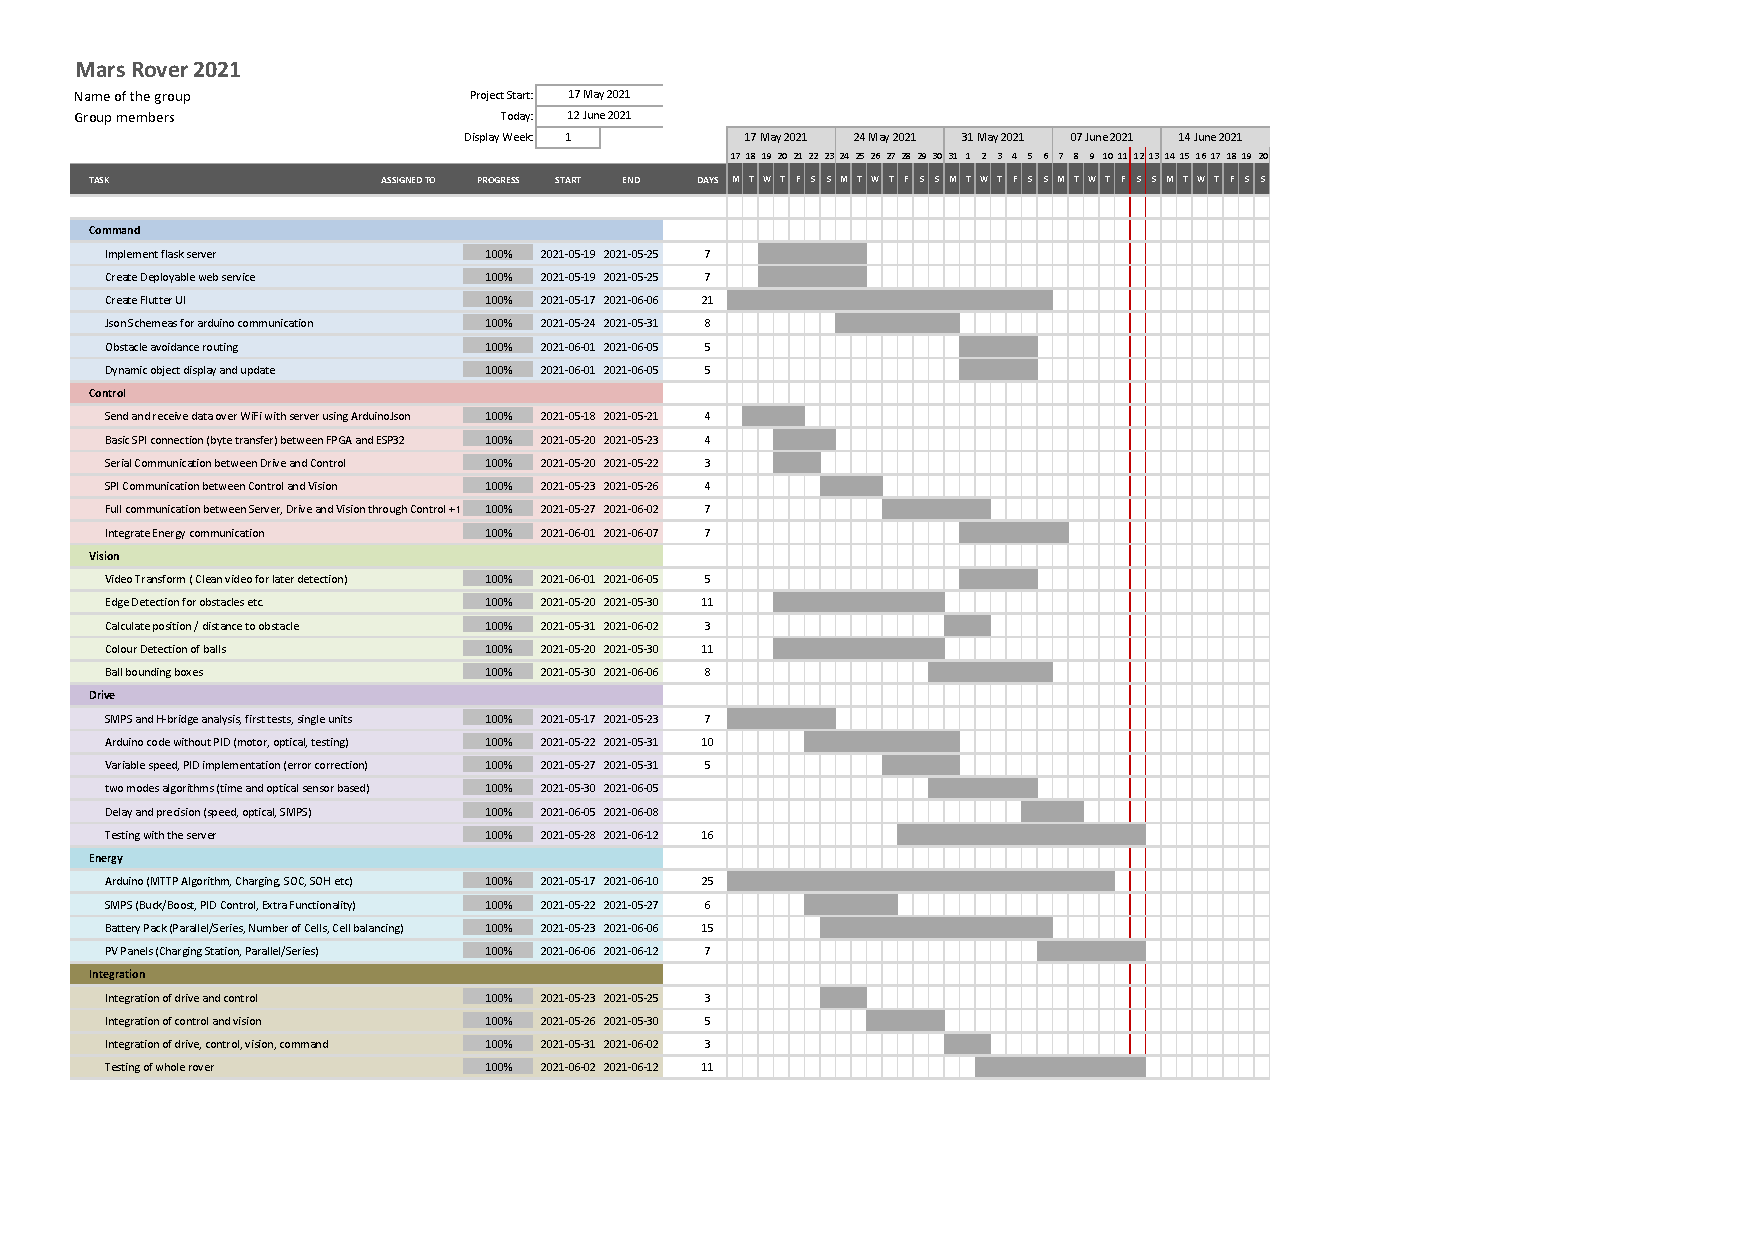
\includegraphics[scale = 0.6,trim={1cm 3cm 8cm 0},clip]{GanttChart.pdf}
    \caption{Gantt Chart}
    \label{fig:GanttChart}
\end{figure}

The Gantt chart shows project progress from the second week onwards. In week 2, it was planned to work on the basic functionalities of each module e.g. the server for the command module, communication between ESP32 and the server, control of the motor based on data from the optical sensor. In week 3, the basic functionalities were completed and more sophisticated functionalities were considered. By the end of week 4, the design of each module was finalised. The focus of week 5 was testing of the full rover with the final versions of each module. 
 
From the second week on-wards, bi-weekly meetings were held. At the beginning of each week, we held a 45-minute meeting. Each member would take 5 minutes to update the group on their progress on the targets set for the previous week, discuss any issues they found and set new targets for the week. Midway through the week, we had a brief 20-minute meeting to check in on everyone’s progress and give the opportunity for the members to bring up any problems or difficulties they might have run into and adjust plans accordingly.
 
The productivity software Notion was also used for each member to make notes of their initial design process, development and testing. It provided an easy method to share progress with the rest of the team. The shared calendar was used to set dates of meetings and mark internal deadlines. A GitHub organisation was created and used for version control for all modules.

\newpage
\section{Design Process}
\subsection{Structural and Functional Design}

Based on the brief given, the following requirement diagram was created. The diagram details the high level requirements of the rover system and the low level functionalities required to achieve them.

\begin{figure}[hbt]
    \centering
    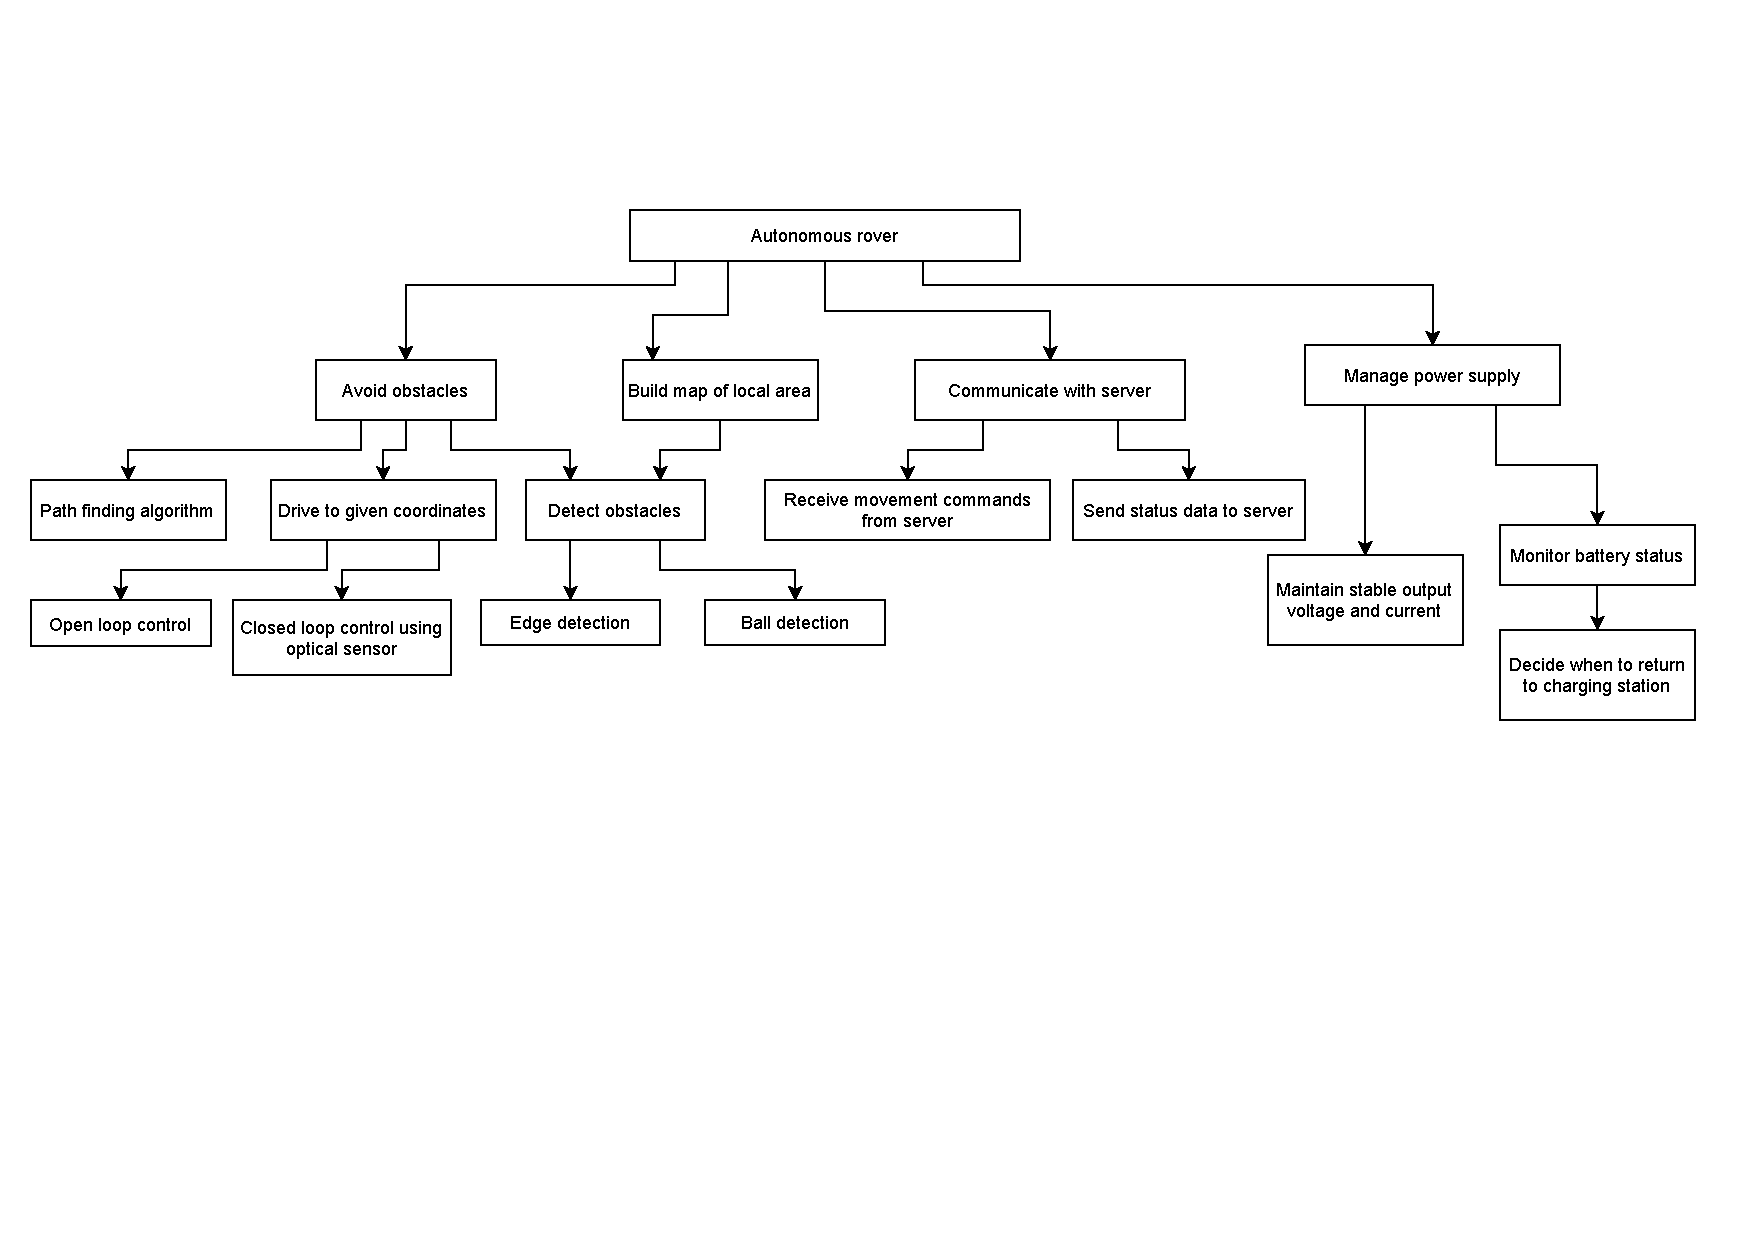
\includegraphics[scale = 0.4, trim={0cm 8cm 0cm 3cm},clip]{Requirements.pdf}
    \caption{Requirement diagram}
    \label{fig:RequirementDiagram}
\end{figure}

The structural design for the full rover system is shown below. The subsystems of the rover system are shown with their internal components and the interactions between different components of different subsystems are drawn out. 
\begin{figure}[hbt]
    \centering
    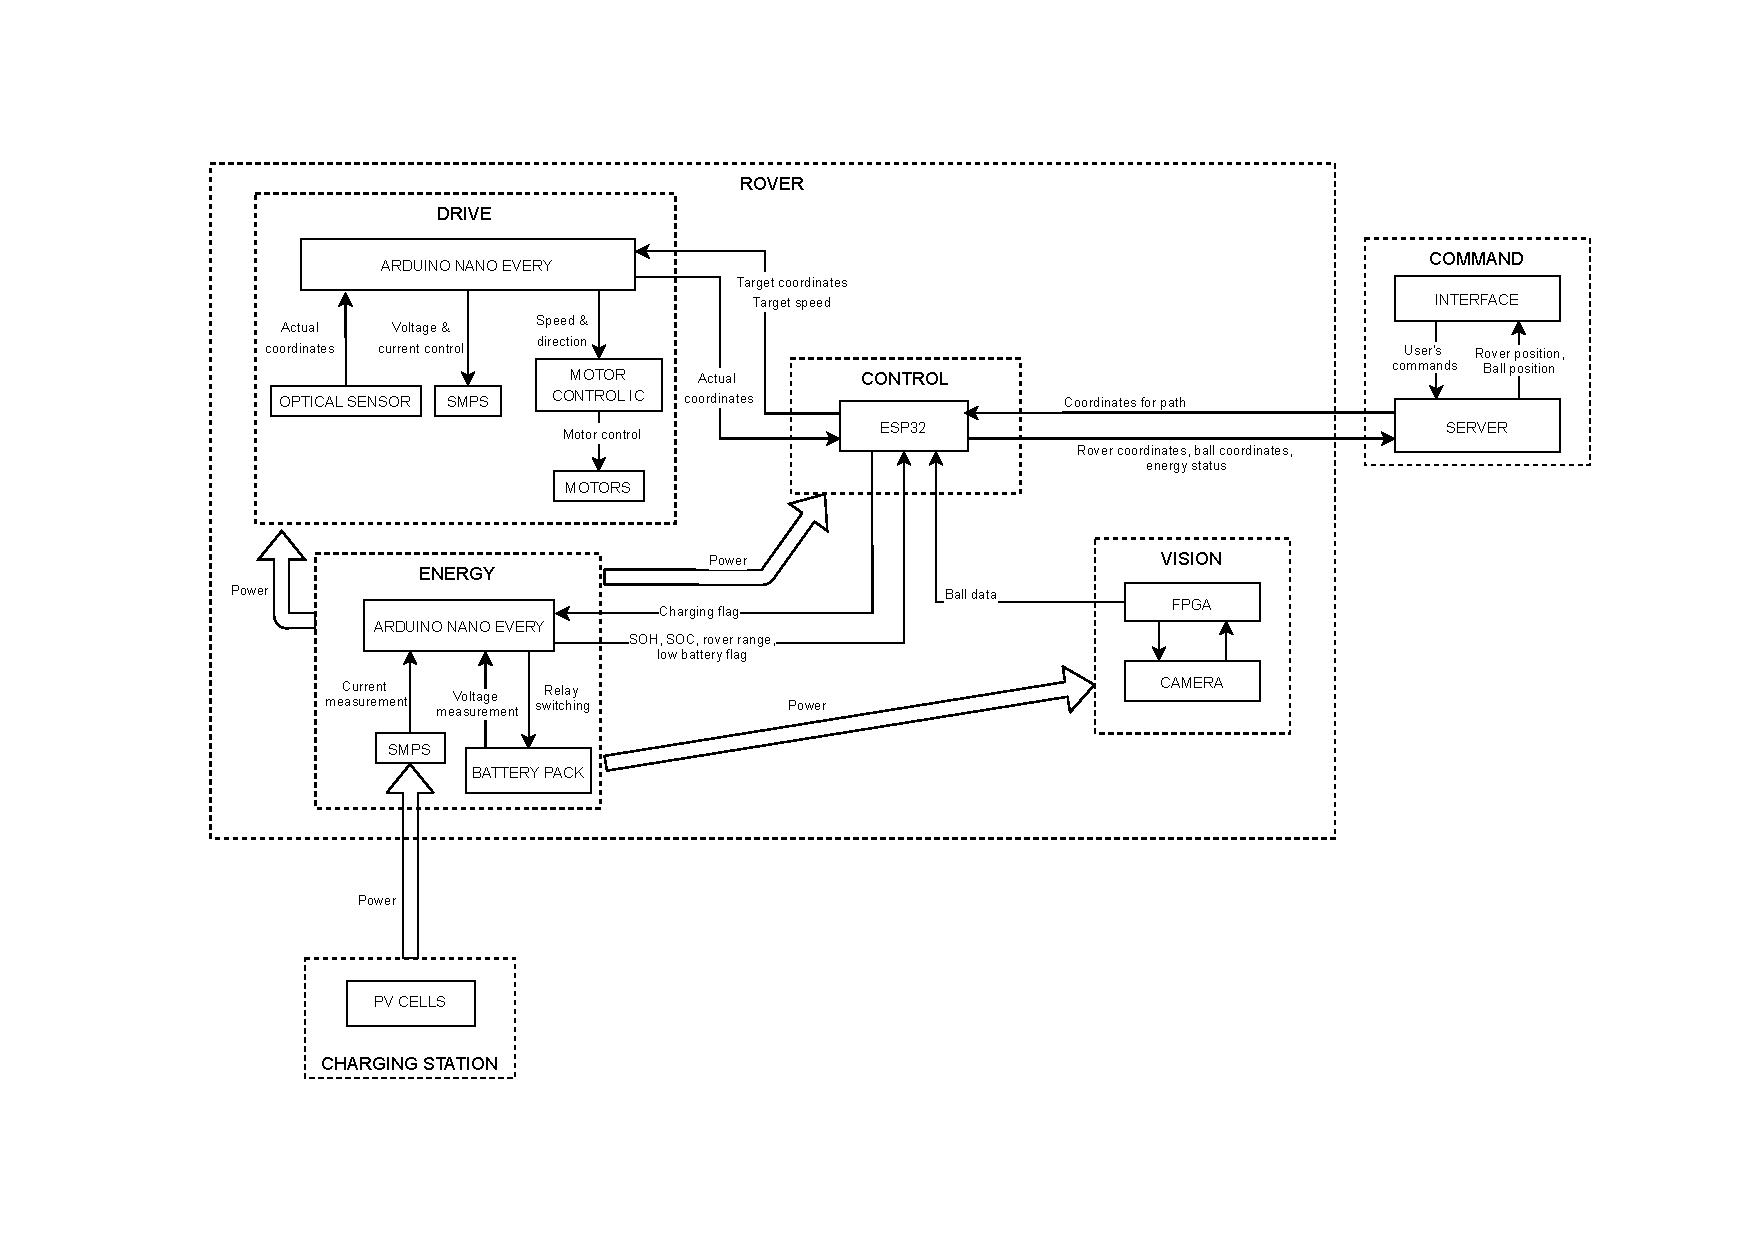
\includegraphics[scale = 0.5, trim={3cm 2cm 2cm 2cm},clip]{StructuralDiagram (1).pdf}
    \caption{Block diagram showing structural design of rover system}
    \label{fig:StructuralDesign}
\end{figure}

The interactions between the rover system and external actors are shown in the diagram below.
\begin{figure}[hbt!]
\centering
  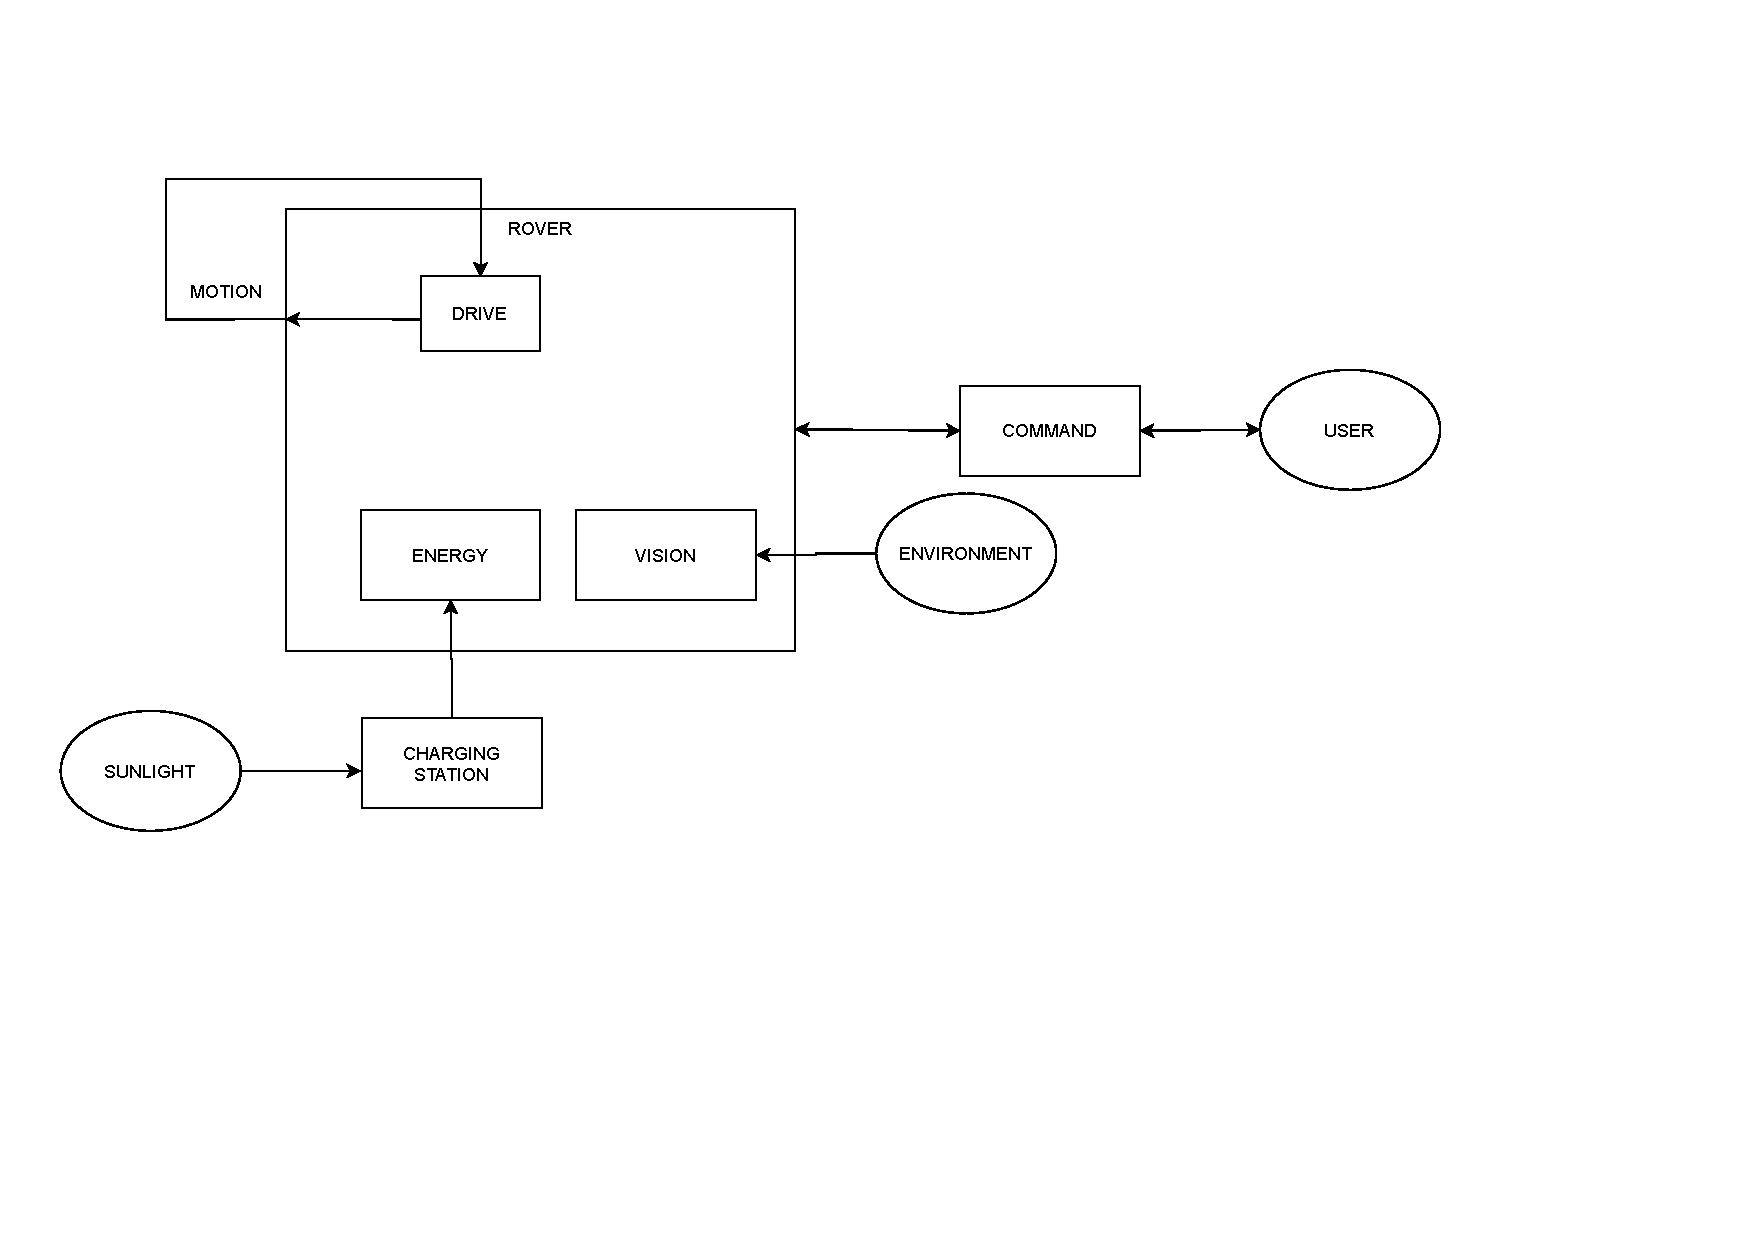
\includegraphics[scale = 0.28, trim={0, 6cm, 0, 3cm},clip]{Context.pdf}
  \caption{Diagram showing interactions between rover system and external actors}
  \label{fig:ContextDiagram}
\end{figure}


\subsection{Problem Definition and Design Criteria}

\subsubsection{Drive}

For the drive subsystem, the following were identified as the functional requirements to be implemented: 
\begin{enumerate} %\itemsep-0.2em
    \item Translate the commands from the control unit into movement instructions for the two motors, in terms of angle and distance to be computed
    \item Move the rover to the specified point in the coordinates system, controlling the speed and direction of the motors via the setting of the SMPS and H-bridge parameters in the Arduino code
    \item Track the movements computed and thus deduce the rover location using the data provided by the optical sensor
    \item Send the location, speed, and orientation data back to the server, communicating the end of the executed instruction
\end{enumerate}
In accordance with these requirements, the design criteria on the base of which our design was evaluated were the following:
\begin{enumerate}
 %\itemsep-0.2em
    \item correct functionality with respect to the requirements
    \item optimal moving algorithm to compute the fastest route in the smallest amount of time
    \item precision of the movements with a 10\% accepted error in the tacking of the location, due to the optical sensor limits
\end{enumerate}
The main structure of the drive subsystem could be divided into two main elements, the two motors and the optical sensor.

\textbf{Motors}

The main elements we had to focus on were the functionality of the SMPS and H-bridge, and the design of a control algorithm to be implemented in the Arduino. For the first part, an analysis of the relevant material and specifications had been pursued and, in a second moment, it was decided with the energy unit to use a reference voltage of 5V for the output of the SMPS (input of the H-bridge). After some testing with a maximum duty cycle for the SMPS, it was concluded that this reference voltage would lead to a maximum speed of the wheels of 60 rpm, a satisfactory speed for the rover to use and yet small enough for the optical sensor data to be reliable.

\textbf{Optical sensor}

The optical data had to be analysed via the Arduino for different surfaces and, after adjusting the lens of the optical sensor, we managed to achieve an increase in the quality of the distance measurements. However, after some testing, we concluded that the sensor would give reliable data only for specific surface and an alternative way of computing the rover’s change in location had to be implemented for surface too uniform or reflective. 

In general, the drive unit development consisted in the coding of Arduino programs comprehensive of all the functional requirements of the subsystem, alongside measurements of the SMPS parameters and wheels’ movements. Due to a large number of Arduino code, Github was found to be a useful tool to keep track of the process and provide the integration unit with updated code for the parallel testing of the whole rover. 

\newpage

\subsubsection{Energy}
The energy subsystem can be split into 4 top-level sections which all combine to provide battery power and charging to the rover. These can then be broken down into smaller subsections which are more manageable and easier to test individually (Table \ref{tab:EnergySpec}). This also allows for more unique features to be added later on in the process. 

\begin{table}[htp]
\renewcommand{\arraystretch}{1.3}
 \centering
\begin{tabular}{@{}cll@{}}
\toprule
\multicolumn{1}{l}{Section}                       & Criteria          & Description \\ \midrule
\multirow{8}{*}{Arduino}                          & Data Collection   & \parbox{0.61\linewidth}{The current and voltage should be recorded continuously for safety}            \\
                                                  & Charge Strategy   & \parbox{0.61\linewidth}{Try to get near maximum possible capacity out of cells}            \\
                                                  & SOC Estimation    &  \parbox{0.61\linewidth}{Real time percentage capacity of the battery via coulomb counting}           \\
                                                  & SOH Maintenance   &  \parbox{0.61\linewidth}{Provide balancing of the cells and an estimation of the SOH}           \\
                                                  & PV MPPT algorithm &  \parbox{0.61\linewidth}{Get the maximum amount of power out of the PV Panels}           \\
                                                  & Communication     & \parbox{0.61\linewidth}{Transmit and receive data from Control}            \\
                                                  & Cell Safety    & \parbox{0.61\linewidth}{$I_{In}^{Max} = 250mA$, $I_{Out}^{Max} = 500mA$, $V_{Bat}^{Max} = 3.7V$, $V_{Bat}^{Min} = 2.3V$}            \\
                                                  & Rover Range     & 
                                                  \parbox{0.61\linewidth}{Work out Rover range from Drive current and speed} \\\midrule
\multicolumn{1}{l}{{\multirow{3}{*}{SMPS}}}       & Charging Buck/Boost        & \parbox{0.61\linewidth}{PV voltage                                             lithium-basedtepped down to battery voltage}            \\
                                                  & Discharging Buck/Boost    & \parbox{0.61\linewidth}{Battery voltage stepped down to motor control voltage} \\ 
                                                  & Drive Current Required &
                                                  \parbox{0.61\linewidth}{$I_{Drive}^{Max}$ = 550mA} \\ \midrule
\multicolumn{1}{l}{\multirow{2}{*}{Battery Pack}} & Number of Cells   &  \parbox{0.61\linewidth}{2}           \\
\multicolumn{1}{l}{}                              & Configuration     & \parbox{0.61\linewidth}{Series to allow to better current limitation ($V_{Nominal}$ = 6.4V)}            \\ \midrule
\multicolumn{1}{l}{{\multirow{3}{*}{PV Panels}}}                     & Configuration     &  \parbox{0.61\linewidth}{2x2 (Two in series then in parallel)}           \\ 
                                                  & Usage &
                                                  \parbox{0.61\linewidth}{A charging station setup in a sunlit area} \\ \bottomrule
\end{tabular}
\caption{\label{tab:EnergySpec} Energy Specification}
\end{table}

\textbf{Design Philosophy}

The energy subsection would require a lot of initial research into lithium-based cells (LiFePO cells were provided) as these have never been covered as a module. A document was made which collated the various amounts of research into cell charging/discharging, safety and PV panels. Then a process of simple testing ensued to characterise some of the cells and PV panels. After this was finished, the direction to take became clearer and work based upon the Gantt diagram (\ref{fig:GanttChart}) began. The aim was to investigate the variety of options available which would allow me to pick and choose the best. This did lead to a number of dead-ends but in many cases, a lot was learned from these and subsequently improved on the overall design.

Due to the large amounts of code required for testing, a number of files were made which would be uploaded to Github. A final Arduino program was made towards the end of the project which could combine all the functions from the various files. These will have been individually tested to ensure they work. Ideally, a final test would also be performed but due to possible defects in the cell supply, this was never realised.

\newpage


\subsubsection{Vision}
The function of the vision system was broken into three general objectives of which the team agreed the system should achieve (See objectives below). We agreed aspects like rover position and pathfinding would be better tackled by different subsystems. The following diagram shows the three main functions of Vision.

\begin{figure}[hbt!]
    \centering
    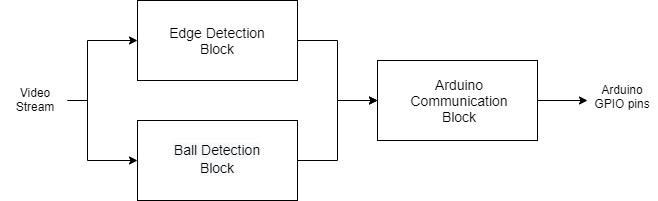
\includegraphics[scale=0.35]{HighLevelDesign.jpg}
    \captionsetup{justification=centering}
    \caption{High Level Block diagram}
\end{figure}

\smallbreak
After this high-level design, each objective was broken down into a series of smaller targets with several criteria which the subsystem would have to meet to successfully accomplish its high-level functionality. 
\smallbreak
\textbf{Ball detection:}

The diagram outlines a basic strategy for approaching the detection of balls through a process of highlighting, filtering and calculating. Each ball occupies its own spectrum of colours and in varying brightness conditions this spectrum can be highlighted so that the maximum and minimum pixels of balls can be determined. Each block was designed to be testable by certain criteria so its success can be verified to ensure the entire block is functioning. 

\textbf{Edge detection:}

By calculating the luminance space of the image one can observe the brightness of each pixel which after the
application of a Sobel filter can be used to produce the edge space. This edge space can then be highlighted
using a threshold. Each block was designed to be testable by certain
criteria so its success can be verified to ensure the entire block is functioning.

\textbf{Communication:}

This block facilitates communication between the Arduino ESP connected to the FPGA pins. It will utilise an agreed method to transfer data one way to the Control subsystem. All variables calculated in the analysis of the vision data will be relayed to it.


\begin{figure}[!htb]
    \centering
    \begin{minipage}{.33\textwidth}
        \centering
        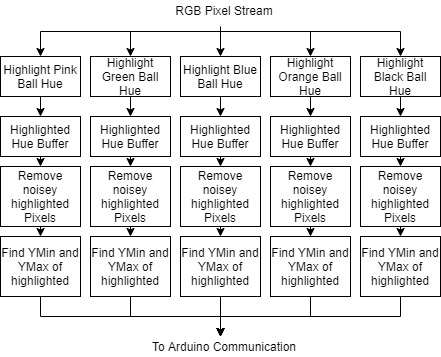
\includegraphics[width=0.8\linewidth, height=0.2\textheight]{BallDetection.jpg}
        \caption{Ball detection overview}
        \label{fig:BallDetectionOverview}
    \end{minipage}%
    \begin{minipage}{0.33\textwidth}
        \centering
        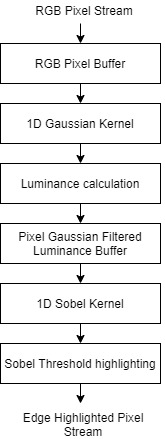
\includegraphics[width=0.4\linewidth, height=0.25\textheight]{EdgeDetection.jpg}
        \caption{Edge detection overview}
        \label{fig:EdgeDetectionOverview}
    \end{minipage}%
    \begin{minipage}{.33\textwidth}
        \centering
        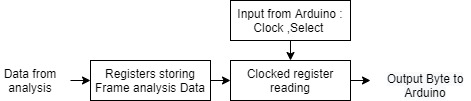
\includegraphics[width=1\linewidth, height=0.08\textheight]{ArduinoComms.jpg}
        \caption{Arduino Comms overview}
        \label{fig:ArduinoComms}
    \end{minipage}%
\end{figure}


\newpage


\textbf{Leaving us with the final design criteria list as such :}

\begin{enumerate}
\itemsep0em
  \item Detect All five balls independently. 
        \begin{enumerate}
            \itemsep-0.2em
            \item Consistently highlight pixels belonging to balls in a plain environment.
                \begin{enumerate}
                    \itemsep-0.2em
                    \item Highlight the intended colour of the ball and no others.
                    \item Eliminate (Do not highlight) the environment that is not the intended ball.
                \end{enumerate}
            \item Filter/Ignore noise data that may exist in the image.
                \begin{enumerate}
                    \itemsep-0.2em
                    \item Successfully remove any data that has been highlighted incorrectly when isolating the ball. 
                \end{enumerate}
            \item Accurately finds the minimum and maximum bounds for balls in the environment.
                \begin{enumerate}
                    \itemsep-0.2em
                    \item Ensure associated Ymin and Ymax are accurate through visual confirmation. 
                \end{enumerate}
        \end{enumerate}
  \item Detect obstructions such as unknown visual data.
        \begin{enumerate}
                    \itemsep-0.2em
                    \item Reveal all Horizontal edges in an image through highlighting
                    \item Extract meaningful depth data from highlighted edges.
        \end{enumerate}
  \item Relay information on detected objects to Control subsystem for further processing.
        \begin{enumerate}
            \itemsep-0.2em
            \item Instantiate a memory that can store all data from analysis of current frame. 
            \item Relay data gathered and calculated in an agreed format to Control subsystem.
            \item Check relayed data is accurately received on the Command / Control subsystem. 
        \end{enumerate}
\end{enumerate}

\textbf{My development philosophy/process was the following:}

I aimed to recursively improve my design and implementation to ensure a robust and flexible subsystem that could adapt to any new criteria, tests or functionality the team agreed upon as the project progressed. This meant I would follow a development cycle illustrated below.

\begin{figure}[hbt!]
    \centering
    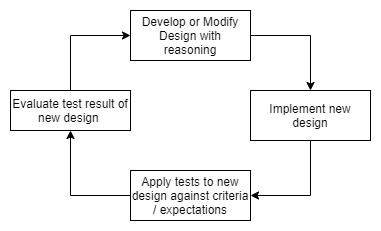
\includegraphics[scale=0.60]{FlowOfDesign.jpg}
    \captionsetup{justification=centering}
    \caption{Subsystem Development Process}
\end{figure}

The development of my system would all take place upon the DE-10 FPGA and camera provided based on the demo project provided. All development was limited to the EEEImgProc.v file where I implemented all Verilog code necessary to meet my design requirements. Any hardware utilised was initialised here or modified in the project QSYS. I aimed at utilising minimal hardware/implementations to develop the subsystem meaning I often implemented designs in Verilog rather than choosing pre-existing library hardware. This was done to reduce issues when debugging and ensure I was not incorporating functionality that was not necessary for my subsystem.




\newpage


\subsubsection{Command}
The rover command module was designed to provide two main functions. Firstly, it had to provide an interface to allow the user to send commands to the rover in different formats and provide information back to the user with regards to the rover's position and sensor data. Secondly, the module had to provide drive commands to the rover based on the user input and on the vision data sent to it from the rover. 
\smallbreak
The different types of commands that we decided to allow the user to send are as follows:
\begin{enumerate}
  \item Commands in the form of a coordinate relative to the rovers current position, with the rover deciding the best route to reach the destination.
  \item Direct commands such as move forward and turn that the rover follows exactly.
  \item Commands to move to a given ball and search for it if its position is unknown. 
\end{enumerate}
The information that would be sent back to the user can be broken down as follows:
\begin{enumerate}
  \item Provide a visual indication of the position of any detected balls relative to the rover position.
  \item Provide an indication of the current charge and battery health of the rover.
  \item Provide a list of the commands the rover still has to complete.
  \item Display the current drive mode that the rover is in.
  \item Display depth data for any object in front of the rover.
\end{enumerate}
In order to allow these requirements to be filled a map-based system was decided upon, this would allow the user to easily click on a position that they desired the rover to move to whilst also displaying the current position of any balls within the same format. In order to allow for commands to be entered a textual input format would also be needed. In addition to ball detection, we also decided to try and find some way of estimating the depth in front of the rover to any obstacle using the difference between two successive frames. It was unclear at the beginning of the project if this would be possible.
\smallbreak
When calculating the actual commands to send to the rover, the command module would use three different modes. Map mode, where the user clicks on the map to send a coordinate, command mode where the user send textual commands and search mode where the user can specify a ball to search for.
\\
It was decided that whenever the rover completed a movement sent to it from command, it would send back its change in position and orientation along with any sensor data. This would allow the command module to calculate the new command to send the rover.

\newpage
\subsubsection{Control}

The Control subsystem's main task is to allow fast and efficient data exchange between the server and the rover. This process can be broken down into:
\begin{itemize}
    \item Collect processed data provided by the relevant subsystems
    \item Send the collected data to the server for analysis
    \item Receive data back from the server and forward it to the relevant subsystems
\end{itemize}

The Control subsystem should take advantage of: \newline
\smallskip
\textbf{Wireless communication} Wireless communication is needed to exchange information with the remote server. \newline
\smallskip
\textbf{Wired communication} Local communication is needed to provide local fast information exchange between the various subsystems. Some data can be processed locally and does not need to be sent to the server.

\begin{figure}[hbt!]
  \begin{minipage}[b]{0.44\textwidth}
    \centering
    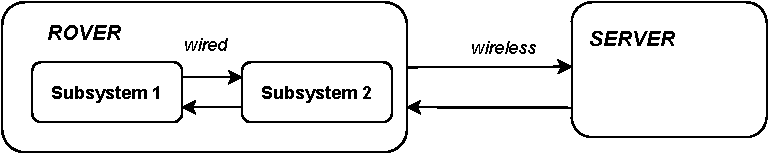
\includegraphics[scale = 0.73]{Server_to_rover_v2.pdf}
    \caption{high level Rover/Server communication}
    \label{fig:server_to_rover}
  \end{minipage}
  \hfill
  \begin{minipage}[b]{0.44\textwidth}
    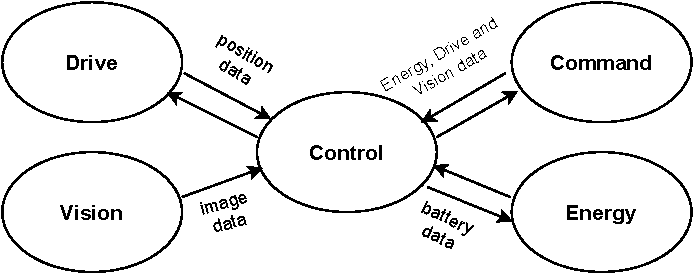
\includegraphics[scale = 0.7]{Finial_Comms_Highlevel.pdf}
    \caption{high level subsystem communication}
    \label{fig:subsystem_communication}
  \end{minipage}
\end{figure}

The control subsystem needs to communicate with every other subsystem via a suitable communication protocol. 
This task can be broken into smaller sub-tasks:
\begin{itemize}
    \itemsep-0.2em
    \item Communication with the Command subsystem
    \item Communication with the Drive subsystem
    \item Communication with the Vision subsystem
    \item Communication with the Energy subsystem
\end{itemize}
In particular, the communication between the subsystems should satisfy the following design criteria:
\begin{itemize}
    \item Communication should be \emph{fast} (i.e. communication delay for transferring data should be less than 100ms )
    \item Communication should be \emph{reliable} (i.e. corruption of data due to external factors should be minimized)
\end{itemize}

Furthermore, the communication protocol should be chosen taking into account the amount of information exchanged with other subsystems (payload size) and whether the communication is unidirectional or bidirectional. A summary of these parameters can be found in the following table:


\begin{table}[hbt]
\centering
\renewcommand{\arraystretch}{1.3}
\begin{tabular}{@{}llll@{}}
\toprule
Subsystem & Data   exchanged                & Payload size & Communication   mode                                       \\ \midrule
Vision    & Processed   image data          & Large        & Unidirectional  $\vert$ Vision $\rightarrow$ Control            \\
Drive     & Position data                   & Small        & Bidirectional  $\vert$ Drive $\leftrightarrow$ Control   \\
Energy    & Battery data                    & Small        & Bidirectional  $\vert$ Energy $\leftrightarrow$ Control  \\
Command   & Energy, Drive   and Vision data & Very Large   & Bidirectional  $\vert$ Command $\leftrightarrow$ Control \\ \bottomrule
\end{tabular}
\caption{Communication Summary}
\end{table}




\newpage

\section{Design Implementation}

\subsection{Drive}

 Our development and implementation strategy consisted of three main steps:
 \begin{enumerate}
     \item \textbf{First, functional model:} A simple moving algorithm was coded based on the optical sensor to meet the basic functional requirements. This model was based on a feedback system that could correct the angle error first and the distance error secondly. Both were computed by comparing the optical sensor and the target coordinates. This model was tested in its functionality and its compatibility with the control unit was checked to have a first general working model. 
    \item \textbf{Further, optimized models:} More features were progressively added to the main body of the code to optimise the performance, both in terms of time needed to reach a given location and precision of the movement computed and tracked. At this stage, the following additions were considered and tested:
	     \begin{itemize}
            \item Arch trajectory (instead of turning on the spot and moving forward)
	        \item Time-based model as an alternative to the optical sensor based one (to avoid the error caused by the optical sensor when the quality of the data is low)
            \item Variable speed implementation to be decided by the server
            \item PI controller for the speed
            \item Calculation of the current at the input of the SMPS to compute the power drawn by the drive unit
            \item PI controller for the trajectory
        \end{itemize}
    On top of the functional testing, for each further model developed, a series of systematic measurements were conducted to evaluate the actual improvement in performance against the ideal behaviour expected.
    \item \textbf{Final model decisions:} The different performances were compared against each other in terms of error precision and time needed to compute a given path. Following a general discussion with the other members of the group, the decision on which model to use was based on the priorities agreed in accordance with the needs of the vision and command units. 
 \end{enumerate}



\textbf{ a.	Optical sensor-based model:}

This first model was designed with the idea of using the data from the optical sensor to implement a closed-loop controlled system in which the location of the rover is adjusted based on the angle and distance measurement. After the first functional tests of the sensor, we realised that the coordinates sent to the Arduino are represented in polar form: x = angle computed, y = distance computed. We decided to use polar coordinates throughout the program for more clarity. A detail to be noted is that those coordinates represent the movements of the optical sensor, and not of the centre of the rover itself.

\textbf{Moving algorithm:} The moving algorithm implemented consisted of four states (figure 7): 
\begin{itemize}
    \item The OFF state, during which the rover does not move. Here the code is set up and the new distance and angle target are defined. The first time the code will be run, or any other time in which no movement is required, the distance and angle will be both 0. In this case, he state will automatically go to MAX MOVEMENT, waiting for a new instruction.
	\item The TURN state through which the rover rotates until the angle error between the coordinates of the sensor and the target are smaller than the maximum angle error (set to be 5° for the initial testing). In this state, the motor will turn in opposite directions at a fixed equal speed. The direction of the tuning of each will be in accordance with the sign of the angle to be computed (positive angles the left wheel moves forward and right backwards, vice versa for negative angles). The angle is scaled to be in the range of -180° to 180°.
	\item The MOVE state, where once the rover is set in the correct orientation, it will start moving forward until the difference between the distance measured by the optical sensor and target distance is smaller than the maximum accepted error (1cm for initial testing)
	\item The MAX MOVEMENT state: The rover will continue to loop between adjusting the distance and the angle until their respective errors are negligible (ideally 0). At this point, the system will be in the state of maximum movement and both motors will stop. During this, the angle and distance computed (from the optical sensor) are sent to the server. The new instruction is received and scaled to the unit and range of the distance and angle. After the transmission and reception are completed, all the relevant variables are reset, and the state is set to OFF.
\end{itemize}

\begin{table}[hbt]
\centering
\renewcommand{\arraystretch}{1.3}
\begin{tabular}{@{}lll@{}}
\toprule
State & Motors                     & Task                               \\ \midrule
OFF            & stop                                & Set up   instructions                       \\
TURN           & Maximum speed,   opposite direction & Reach the   angle target                    \\
MOVE           & Maximum speed,   same direction     & Reach the   distance target                 \\
MAX MOVEMENT   & stop                                & Send location   and receive new instruction \\ \bottomrule
\end{tabular}
\caption{Moving Algorithm}
\end{table}
 
 \begin{figure}[hbt]
     \centering
     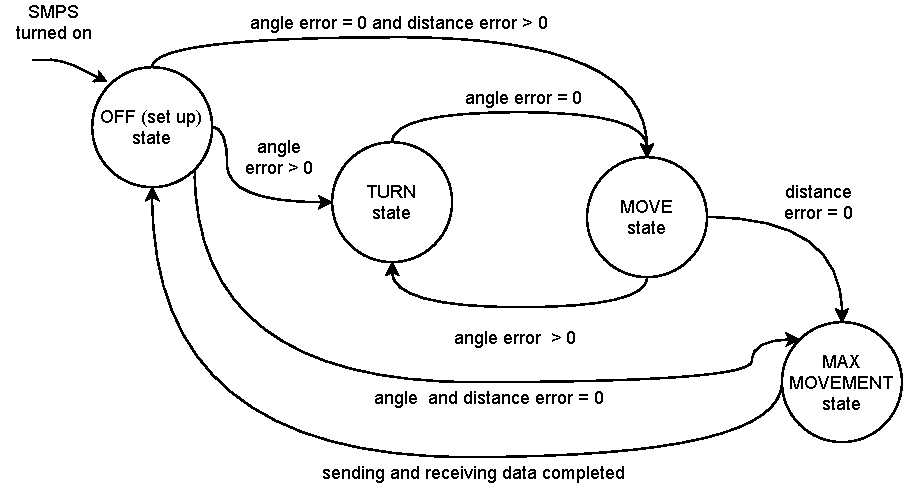
\includegraphics[scale = 0.8]{movestate.pdf}
     \caption{Moving algorithm state machine}
     \label{fig:my_label}
 \end{figure}
\textbf{Variable speed:} The implementation of variable speed seemed to be an important feature that could be used to enhance the performance of the movements. More freedom of choice would be available on the command side of the rover. This was implemented by tuning the value of the PWM (Pulse Width Modulation) input from the Arduino to the gate of the MOSFETs of the H-bridges. Instead of using a digital wire, an analogue wire with values from 0 to 255 was used to control the voltage level perceived by the motor and, consequently, their speed. 

\textbf{Arch trajectory:} The initial idea was to implement a different type of trajectory. An arch movement had been implemented to substitute the “turning on the spot and the then moving straight” procedure. Hence the rover could turn while moving. This model was then tested and, although the functionality was correct, the loss in speed due to the slowing of the wheels (against a constant maximum speed for the previous model) did not justify it's implementation. The original model was already extremely precise and considerably easier to control and track. It was therefore decided not to pursue this model.

\textbf{PID controller:} A model of a PID controller was designed and included in the main code. This was implemented with the idea to better control the precision of the movements when turning or moving forward. The controller for the angle correction compared the angle measured and the target angle. It would then tune the speed of the turn accordingly. The distance controller worked in the similar way, but adjusting the speed used to move forward instead. The expected behaviour of this model was to progressively increase the speed to the maximum and then decelerate when approaching the target to better control the precision of the arriving point. The gains of the controller were progressively tuned, with exception of the differential one, which did not influence the performance significantly during tuning. 

Another version of the PI was also considered to control the trajectory instead (making the rover go backwards in case of overshoot). However, this would have not increased the performance of the rover since the feedback given by the optical sensor was observed to be working fast enough to not cause any considerable overshoot. Furthermore, the logic of the optical sensor-based model already worked so that if an error in the angle emerges, it will be automatically be corrected by a turn in the opposite direction.

\textbf{b.	Time-based model:}

After comprehensive testing of the optical sensor-based model was concluded, there were certain limitations in the optical sensor that could not be avoided: the quality of the data created by the sensor would decrease beyond an acceptable level when the surfaces on which the rover traveled were too uniform, translucent or of a light colour. This is because the sensor is not able to properly detect the movement computed. Therefore, it was decided that there is need of an alternative model to be used in these edge cases. This model would not use the feedback of the sensor to calculate the distance and angle to be computed. Instead it would calculate a time of execution for the turning and moving forward. These two values are calculated in the code based upon the maximum speed of the wheels measured for the rover (60rpm) and the distance or angle to be computed.
Being aware that this a more empirical and imprecise way of proceeding, this algorithm is to be considered as only a back-up model for when the quality of the optical data is extremely low and could lead to major errors in the feedback.

\textbf{Final model:}

In accordance with the results from the testing, a final more optimised model was created integrating all the successful features in a single program.
The logic of the code is summarised in figure 8 and includes the following elements:
\begin{itemize}
\item 	Error detection and correction: The optical sensor feedback and PI controller check that the direction is right and adjust the movement of the wheels accordingly. This leads to a maximum error within a margin of 5° and 5mm. In general the error was within 10\%.
\item 	Multiple modes to move depending of the quality of the optical data: The optical sensor feedback if the quality is above a certain level (15 stars are usually a recommended level at which the data is reliable; however, by measuring the performance, 10 stars had been observed to still lead to good data quality)
\item 	Speed value of the wheels decided by the server within the range of 5-60rpm. By default the maximum speed is used.
\item 	Input current drawn from the energy unit is computed and the value send to the control unit in order to calculate the power consumed. The input current of the SMPS was computed by the measurement of the output current by the current sensing resistor and the formula $I_(in) = V_(out)*I_(out)/V_(in)$ (for more see energy unit)

\item 	Sending and receiving section implemented via SPI (see control unit)
\end{itemize}

\begin{figure}[hbt]
    \centering
    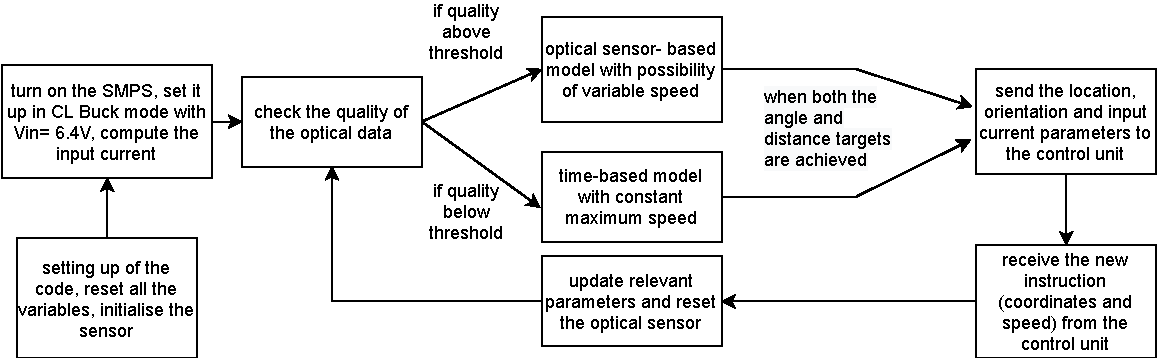
\includegraphics[width = \textwidth]{driveunit_structure.pdf}
    \caption{Final logic of the drive unit}
    \label{figure}
\end{figure}

Furthermore, a few adjustments were made to enhance the performance of the rover as a whole. Taking into account the need of the vision unit specifically: The idea is that the model has to be designed keeping in mind the highest goal of the Mars Rover itself, i.e. to move around in an unknown environment mapping the surrounding. For this reason, we thought that the quality of the images, movements and the precision of the data from the mapping process had to be prioritised over the smoothness of the movements themselves or the simplified communication feedback. Therefore, we decided make the communication between the control and drive unit more frequent by letting the rover send data every 50 millimetres or 20° computed. This has two main benefits: Firstly, the mapping and the obstacle detection given by the vision unit is more accurate since the server has a frequent feedback on the current location; Secondly, if any sudden change in the surrounding environment occurs or the error from the optical sensor accumulates throughout the instructions, the command has the time to process it and adjust the optimal trajectory immediately. This design decision was confirmed after testing the rover and measuring that the delay given by the more frequent transmission of data is very contained (??numbers??).

\subsection{Energy}
\subsubsection{Arduino}

\textbf{Data Collection}

Upon initial testing of the Arduino, it became clear that the analogue inputs fluctuate significantly. To mitigate this for both the current and voltage, a 'moving average' filter was implemented which took the 1000 values before the slow loop and summed them in a cumulative variable. This was then divided by 1000 to get the average.

\textbf{Charge Strategy}

To get the most capacity out of a single cell, a CC/CV (Constant Current/ Constant Voltage) charge strategy was decided upon. This involves charging a cell with a steady current until the maximum voltage is reached. Both the charging current (250mA) and maximum voltage (3.6V) are dictated by the data sheet of the cell in use (Appendix \ref{appendix:Energy}.\ref{fig:CellSpecification}). The cell is then charged using a constant voltage whereby the current slowly decreases as seen during testing in figure \ref{fig:TestCCCV}. This ensures that the maximum cell voltage is not surpassed while still trickle charging the cell to near maximum. The current cut-off was set at 0.1C (50mA) so that the cell would not take an excessive amount of time trickle charging. A PID was used to control both the voltage and current. This changed to a combination of MPPT and voltage PID when the charging station was involved. 

\textbf{SOC}

Measuring the state of charge is difficult in real time due to a range of factors. This includes fluctuations in temperature and the degradation of the cell as the number of charge-discharge cycles increases. The computation power of the Arduino is also another factor to consider and therefore an Enhanced Coulomb Counting method \cite{Ng2009EnhancedBatteries} was decided upon. This will work out the amount of charge going in/out of the cell and thereby the change in the SOC. Therefore, an initial value of the SOC will also be needed. Given the direct relationship between the SOC and OCV (Open Circuit Voltage), a lookup table was extracted from early cell characterisation seen in figure \ref{fig:SOC_OCV}. This is also tightly integrated with SOH Maintenance to allow for auto calibration and integration with the passive balancing algorithm. (Figure \ref{fig:SOCFlow}). 

\begin{figure}[hbt]
    \centering
    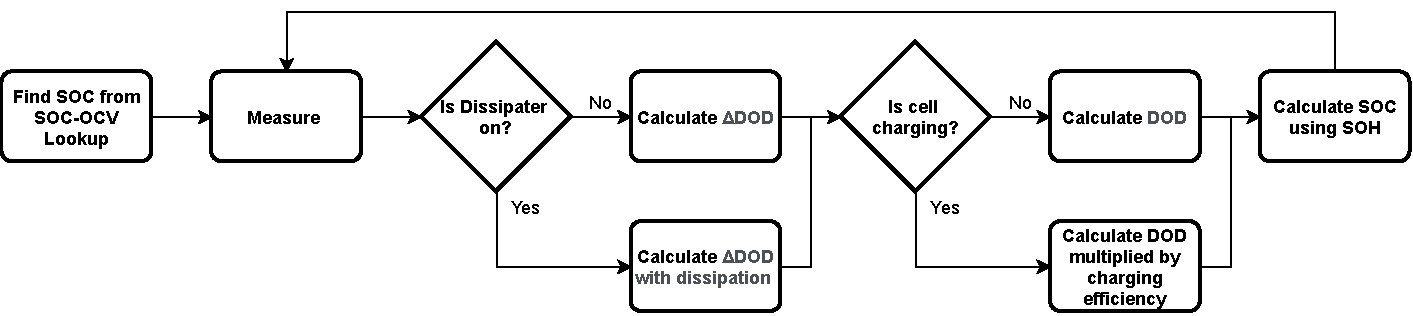
\includegraphics[scale = 0.65]{ColoumbCounting (2).pdf}
    \caption{Top level SOC finding algorithm}
    \label{fig:SOCFlow}
\end{figure}


\noindent\begin{minipage}{.32\linewidth}
\begin{equation}
    SOC = 1 - DOD
  \label{equ:SOC}
\end{equation}
\end{minipage}
\begin{minipage}{.32\linewidth}
\begin{equation}
    SOH = \frac{Q_{Discharge}^{Max}}{Q_{Rated}}
  \label{equ:SOH}
\end{equation}
\end{minipage}
\begin{minipage}{.32\linewidth}
\begin{equation}
    \eta_c = \frac{Q_{Discharge}^{Max}}{Q_{Charge}^{Max}}
  \label{equ:ChargeEfficiency}
\end{equation}
\end{minipage}

In (\ref{equ:SOC}), the state of charge can be represented as a decimal or percentage. It is a measure of the current capacity of the cell. The state of health (\ref{equ:SOH}) is defined as the maximum discharge capacity compared to the rated capacity of the cell. It can also be represented as a percentage of the rated capacity. The charge efficiency (\ref{equ:ChargeEfficiency}) is used to create a more accurate Coulomb counting algorithm whereby the increased capacity needed during charging is accounted for as seen in figure \ref{fig:SOCFlow}.   

\noindent\begin{minipage}{.49\linewidth}
\begin{equation}
    \Delta DOD = \frac{I_{Bat}}{3600*SOH*Q_{Rated}}
  \label{equ:DeltaDOD}
\end{equation}
\end{minipage}
\begin{minipage}{.49\linewidth}
\begin{equation}
    DOD_{(k+1)} = DOD_{(k)} - \eta\Delta DOD
  \label{equ:DOD}
\end{equation}
\end{minipage}

In discrete one second intervals, $\Delta DOD$ (\ref{equ:DeltaDOD}) is seen to be the amount of amp-hours in the sampling period compared to the maximum discharge capacity which has been expanded to include the SOH. During charging, the next value of depth of discharge (\ref{equ:DOD}) decreases with an $\eta = \eta_c$. Conversely, the DOD increases during negative current (Out of cell) with $\eta=1$.

\textbf{SOH Maintanance}

The state of health decreases as the number of charge-discharge cycles begins to accumulate. Hence it is important to track ensuring an accurate Coulomb Counting algorithm. This can be done by calibrating the SOH and $\eta_c$ during a full charge/discharge (\ref{fig:RecalibrationAlgorithm}). This was done during the characterisation of each cell. Ideally this would happen after 1-2 full charge-discharge cycles which would allow the coulomb count to zero itself. To prolong the life of a cell in a battery pack, an SOH maintenance strategy must be employed. This is needed to prevent a single, smaller cell, from restricting the larger cells from charging to maximum capacity. The smaller cell would then degrade at a faster rate than the others leading to a lower overall battery capacity. This strategy involves developing a system to keep the various SOCs at around the same level. There are a range of balancing strategies open to us. The simplest and most effective is passive cell balancing. This involves using dedicated dissipation resistors through which the individual cells can discharge to lower their respective SOC to that of the whole battery pack. This seemed like the most obvious option given the already implemented dissipation resistors in the battery PCBs. The balancing algorithm was then idealized shown by the flowchart in figure \ref{fig:DisAlgorithm}. It should be noted that the cells should stop dissipating when they are within 3\% of its other due to the SOC only being an estimation

\begin{figure}[hbt]
    \centering
    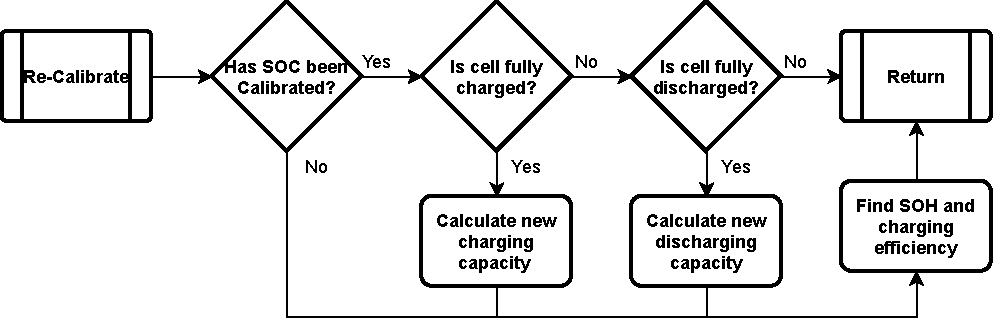
\includegraphics[scale = 0.65]{Recalibration (1).pdf}
    \caption{Re-calibration algorithm}
    \label{fig:RecalibrationAlgorithm}
\end{figure}

\noindent\begin{minipage}{.49\linewidth}
\begin{equation}
    Q^{Max}_{{Charge}_{(k+1)}} = \frac{SOC - SOC_{Init}}{DOD_{Init}}Q^{Max}_{{Charge}_{(k)}}
    \label{equ:NewChargingCap}
\end{equation}
\end{minipage}
\begin{minipage}{.49\linewidth}
\begin{equation}
    Q^{Max}_{{Discharge}_{(k+1)}} = \frac{SOC_{Init} - SOC}{SOC_{Init}}Q^{Max}_{{Discharge}_{(k)}}
    \label{equ:NewDischargingCap}
\end{equation}
\end{minipage}

Equation \ref{equ:NewChargingCap} states that the new value of the maximum charge capacity is the ratio of the actual DOD at full capacity compared to the initial estimated DOD multiplied by the old value for the maximum capacity. Hence, if the real DOD was lower than estimated, a smaller value of charge capacity would be calculated. This can then be used to find a new $\eta_c$ (\ref{equ:ChargeEfficiency}). Similarly, (\ref{equ:NewDischargingCap}) calculates a new discharge capacity by using the ratio of the actual DOD and the initial SOC. This is then applied to the previous value of the discharge capacity. Through this, a re-calibration of the SOH (\ref{equ:SOH}) and $\eta_c$ (\ref{equ:ChargeEfficiency}) can be processed.
\begin{figure}[hbt!]
    \centering
    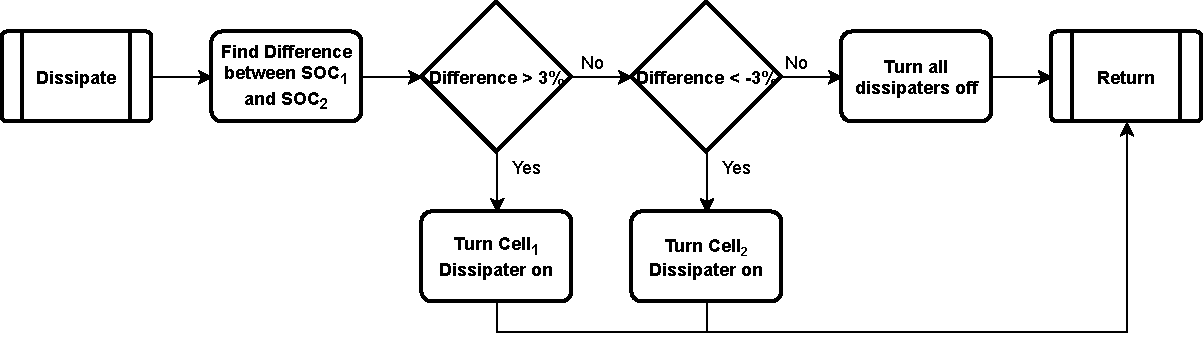
\includegraphics[scale = 0.65]{Dissipate (3).pdf}
    \caption{Dissipation algorithm}
    \label{fig:DisAlgorithm}
\end{figure}

\textbf{PV MPPT Algorithm}

PV panels produce a non-linear voltage-current curve which can vary significantly with temperature and luminosity. This multiplied by the changing efficiency of the SMPS leads to a non-linear, dynamic power curve (\ref{fig:PVvoltage}) which needs to be taken advantage of in order to get the maximum power output. It was decided that Incremental Conductance would be used in the MPPT algorithm due to low fluctuations at the peak. The strategy works by making a linear estimation of the gradient using the past sample value as seen in (\ref{fig:Gradient}) and following the flowchart seen in figure \ref{fig:IncrementalConductance}. A positive gradient would mean that the system is on the left hand side of the peak and vice versa for a negative gradient. The function would then change the duty cycle accordingly to change the impedance of the power supply as seen by the PV panel. These duty cycle 'steps' would be larger the for steeper gradients. The MPPT program also tracks if the irradience has changed which would result in no change in voltage but a change in current. 
\begin{equation}
    \frac{dP}{dV} = \frac{d(VI)}{dV} = I + \frac{dI}{dV} \approx I + \frac{\Delta I}{\Delta V}
    \label{fig:Gradient}
\end{equation}

\begin{figure}[hbt!]
    \centering
    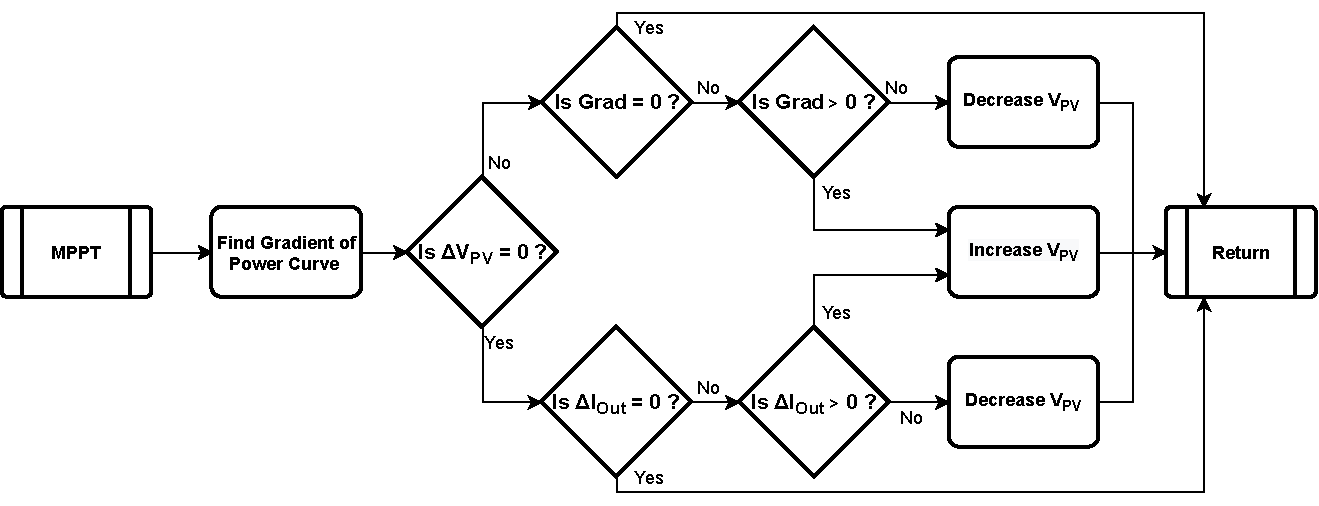
\includegraphics[scale = 0.6]{IncrementalConductance2 (3).pdf}
    \caption{Incremental Conductance Algorithm \quad Source: Adapted from \cite{Choudhary2014IncrementalConverter}}
    \label{fig:IncrementalConductance}
\end{figure}

\textbf{Communication}

Communication between Energy and the rest of the subsystems is important in the reliability of the rover. The SOC, SOH, Rover Range and Low Battery Flag will be sent to control which will relay these to Command. The SOC will be that of the lowest cell and the SOH will be the average of both cells. To get an accurate SOC and Rover Range, the overall current drawn and speed of the rover must be received by Energy. Lastly, Command must send a Charge Flag to indicate that the rover is connected to the solar charging station. 

\textbf{Cell Safety}

The use of LiFePO cells requires stringent safety protocols. Based upon the cell specification (Appendix \ref{appendix:Energy}.\ref{tab:EnergySpec}) and the maximum values in table \ref{tab:EnergySpec}, the energy subsystem will completely shut down and refuse to give power unless the problem is solved. This will be done with the use of relays which will disengage the cells.

\textbf{Rover Range}

The rover range is found using (\ref{equ:RoverRange}). This will provide an estimate given the speed, SOC and current draw. The equation will be adjusted according to the SOH; keeping the estimate accurate as the cycle count of the battery pack increases.   
\begin{equation}
    Range = \left(\frac{Q_{Discharge}^{Max}}{I_{Out}}3600\right) v_{rover} = \left(\frac{SOC \ SOH \ Q_{Rated} }{I_{Out}} 3600\right) v_{rover}      
    \label{equ:RoverRange}
\end{equation}
\subsubsection{SMPS}

\textbf{Initial Top Level Design}

How the Energy subsystem is integrated within the design of the rover is more of a hypothetical problem. The processing on board requires a reliable 5V supply which would require the use of another SMPS to step down the voltage of the cells. In our case, the battery is only used to power the motor control through a connection to Port A of the Drive SMPS as seen in figure \ref{fig:InitalDesign}. The drive current is needed to work out the actual current going through the battery for the SOC and range calculations.

\begin{figure}[hbt]
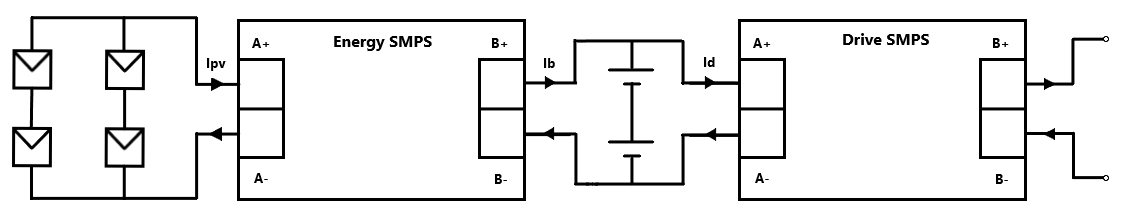
\includegraphics[scale = 0.5]{SMPS}
\centering
\caption{Preliminary design for connection to drive subsystem}
\label{fig:InitalDesign}
\end{figure}

\subsubsection{Battery Pack}

It was decided that safety and good cell maintenance would be a priority when deciding on the configuration of the cells. This led to the series design seen in figure \ref{fig:InitalDesign}. The series battery pack has the advantage that one can always monitor the current going through each cell which can then be used to ensure the battery is not damaged through over charging/discharging. Unfortunately, more than two cells in series is not possible with the SMPS in synchronous mode due to a $\approx 8V$ limit on port A. This is a limitation of the PMOS MOSFET's Gate threshold voltage and more cells cannot be added as the Drive SMPS requires a buck configuration (Hence the PMOS cannot be set as a diode). During series operation, constant voltage mode would be set up on each cell individually to make sure that no cell is overcharged. 

\subsubsection{PV Panels}

One can see the classic characteristic PV curves on figure \ref{fig:PVvoltage}. The PV specification (Appendix \ref{appendix:Energy}.\ref{tab:PVSpecification}) states that PV panel operates at approximately 5V. As seen in figure \ref{fig:InitalDesign}, a 2x2 design ensures that the maximum power point voltage will be above that of the battery pack at around 10V. Like before, the input voltage limit of the SMPS will affect this arrangement. During testing it worked but a series configuration with 4 panels is impossible as the Buck mode is required from the SMPS.

\subsubsection{Final State Machine}

\begin{figure}[hbt]
    \centering
    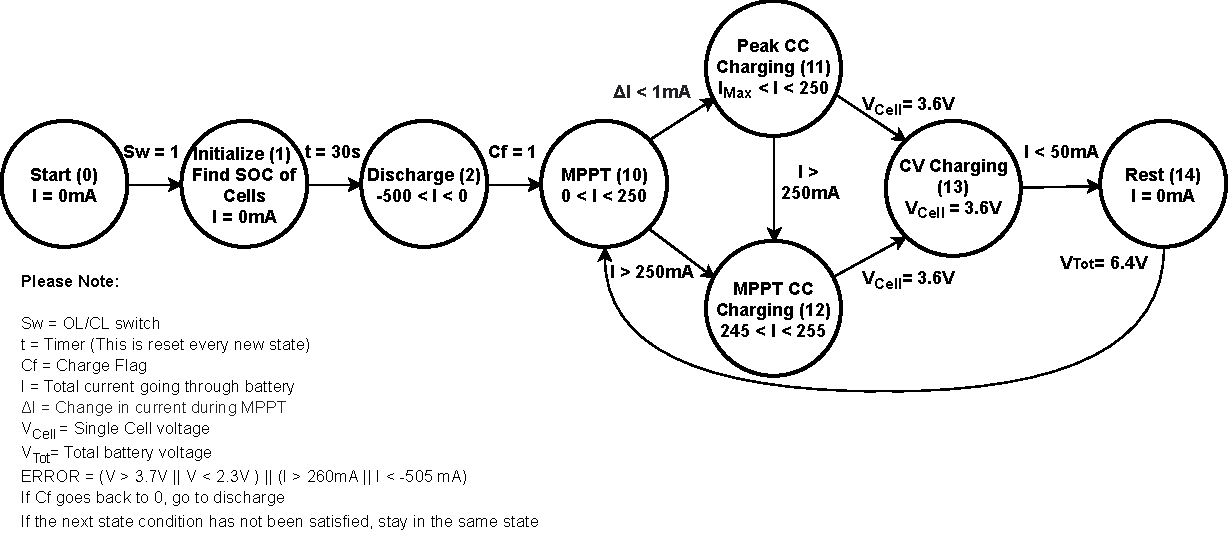
\includegraphics[scale = 0.8]{Final (3).pdf}
    \caption{Final State Machine}
    \label{fig:FinalState}
\end{figure}

The final state diagram can be seen in figure \ref{fig:FinalState}. It should be noted that the various functions providing special capabilities (Dissipation, Communication, etc) stated above run every cycle and so have not been included. Note the dual charging stage, if the MPPT reaches 250mA while trying to get to the peak, it stops and keeps the current approximately at that value by using MPPT and inverse MPPT. Otherwise, the peak of the MPPT is used meaning that it is in operation constantly. It then comes together with the voltage PID. This can be done as the current curve leading up to the 250mA will be linear if the peak is higher than the charging current. Similarly, this will also work if the peak is lower than 250mA as the PID will always decrease. A final circuit diagram can bee seen in Appendix \ref{appendix:Energy}.\ref{fig:FinalCircuit}


\subsection{Vision}

\subsubsection{Edge detection implementation:}

We use edge detection to provide more advanced data for obstacle avoidance and route planning. It is also used to corroborate the hue analysis that occurs in ball detection. This provides us with a more detailed image of the environment. 

Video data is received from the camera as a continuous stream of RGB pixels or frame packet information. The edge detection processes the video stream to highlight the object outline. Each pixel received is in an RGB format where R,G and B are represented by a byte having a value between 0 and 255. 

The first step in the edge detection process is to calculate the luminance of each pixel from its RGB values. Luminance or Luma is an important photo-metric measure describing the brightness of a pixel. It is often used to produce an achromatic image giving us a more meaningful visual space to extract information from. An approximation for the digital CCIR 601 \cite{LumaWikipedia} video standard was used. This value will be between 0 and 255 and be a weighted sum of the R, G, B values of the pixel. 

\begin{minipage}{.49\textwidth}
\begin{equation}
    Y_{601} = 0.299R + 0.587G + 0.114B
\end{equation}
\end{minipage}
\begin{minipage}{.49\textwidth}
\begin{equation}
    Y_{Approx} = 0.375R + 0.5G + 0.125B
\end{equation}
\end{minipage}

An approximation is used as representing specific fractions as series of additions and bit shifts in Verilog introduces a large amount of complexity. It was decided that the small reduction in accuracy was acceptable for our application as later a threshold would be applied which would highlight low and high luminances.

\begin{figure}[hbt]
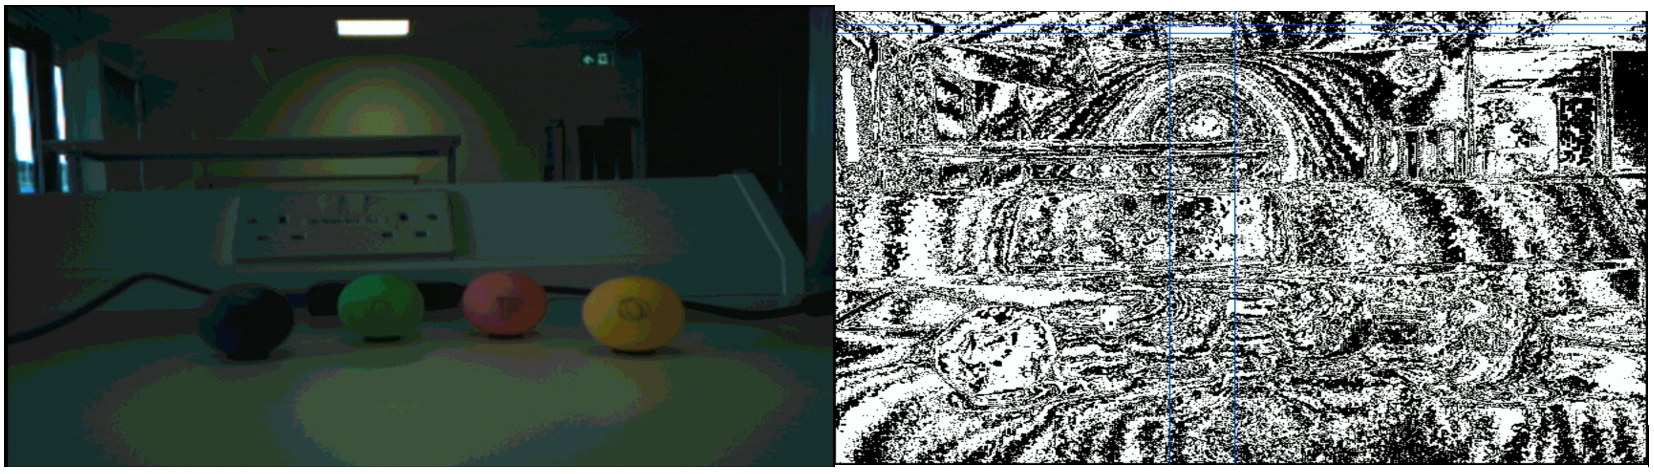
\includegraphics[scale = 0.3]{ExampleLuminance.PNG}
\centering
\caption{Example Luminance image }
\label{fig:LuminanceImg}
\end{figure}


Following the review of the luminance space image, a large amount of speckled noise-like data was observed. Gaussian filtering was used to remove this data to give a smoothed luminance space. This helped in eliminating erratic brightness data that may be present in the luminance space. The Gaussian filtering was accomplished through the convolution of a 1D Gaussian kernel with a series of horizontal pixels and returning a Gaussian value which is the convolution product for that specific pixel. See reference \cite{SpatialSmoothing}

\begin{figure}[hbt]
    \begin{minipage}{.55\textwidth}
    \begin{equation}
        \begin{bmatrix}
        0.006 & 0.061 & 0.242 & 0.383 & 0.242  & 0.061  & 0.006 \\
    \end{bmatrix}
    \end{equation}
    \end{minipage}
    \begin{minipage}{.39\textwidth}
    \begin{equation}
        \begin{bmatrix}
        0.0625  & 0.25 & 0.375 & 0.25  & 0.0625 \\
        \end{bmatrix}
    \end{equation}
    \end{minipage}
    \caption{1D x component Gaussian Kernel (12)  and  approximated version (13)}
\end{figure}

To accomplish convolution the current and previous four values of pixel luminances are stored in a buffer called Gaussian\verb|_|buffer. After storing these values, the sum of weighted values is calculated in the buffer. Weighting is accomplished through bit shifting each luminance value according to its position. The weighting values are again approximated as shown above to an acceptable degree of accuracy. Thus the kernel moves through the image data horizontally. The sum of weighted luminances is then returned as a Gaussian value in a new stream.

\begin{figure}[hbt]
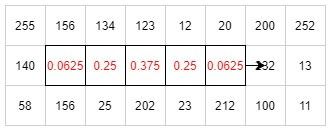
\includegraphics[scale = 0.55]{GaussianBufferjpg.jpg}
\centering
\caption{Gaussian buffer example}
\label{fig:InitalDesign}
\end{figure}

After this convolution I now have a Gaussian filtered luminance video stream which is ready for edge detection

I attempted two methods when implementing edge detection on the Gaussian filtered luminance video stream. The first being a 3x3 kernel applied across and the second a 1X5 horizontal Sobel filter. Both methods had their benefits and drawbacks which will be discussed. 

\textbf{Method 1 - 3X3 Kernel}  - Implementation in Full\verb|_|Sobel branch:

To apply the following kernel it is necessary to have on access the values under the matrix , this stretches across three rows of pixels and three columns.These values are not accessible from the stream so we must create a buffer which stores the previous pixels of the stream making them accessible for the matrix convolution. I attempted to implement this buffer with a bank of registers defined as such:
\begin{minted}{verilog}
reg [7:0] luminance_buffer[2:0][(IMAGE_W-1):0] 
\end{minted}
This stores the RGB values for all pixels in the three rows necessary. However this implementation took exceedingly long to compile. I then attempted a version using a shift register IP block in the QSYS however I stopped developing this method before the shift register was fully implemented as I decided upon using method two.

Thus the matrix convolution will can be calculated as such :
\begin{minted}{verilog}

assign GXSOBEL = (1 * ImageMatrix[2][0] ) + (-1 * ImageMatrix[2][2] ) + 
(2 * ImageMatrix[1][0] ) + (-2 * ImageMatrix[1][2] ) + 
(1 * ImageMatrix[0][0] ) + (-1 * ImageMatrix[0][2] )

assign GYSOBEL = (-1 * ImageMatrix[2][0] ) + (-2 * ImageMatrix[2][1] ) + 
(-1 * ImageMatrix[2][2] ) + (1 * ImageMatrix[0][0] ) + (2 * ImageMatrix[0][1] ) + 
(1 * ImageMatrix[0][2] )

\end{minted}
Finding the square root of the summation is not immediately possible in verilog I imported a SQRT function from the web which I reference here \cite{VerilogROOT} (This way not used in the final implementation however). The value GSOBEL was then calculated from GXSOBEL and GYSOBEL in the following way: 
\begin{minted}{verilog}
assign GSOBELSQUARED = ((GYSOBEL)*(GXSOBEL)) + ((GYSOBEL) * (GYSOBEL)) 
assign GSOBEL = sqrt(GSOBELSQUARED)
\end{minted}

\begin{figure}[!htb]
\begin{minipage}{.49\textwidth}
        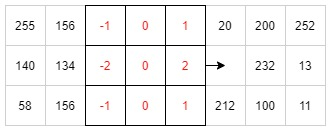
\includegraphics[scale = 0.55]{GX.jpg}
        \centering
        \caption{Horizontal Sobel filter example}
        \label{fig:InitalDesign}
\end{minipage}
\begin{minipage}{.49\textwidth}
        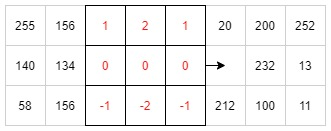
\includegraphics[scale = 0.55]{GY.jpg}
        \centering
        \caption{Vertical Sobel filter example}
        \label{fig:InitalDesign}
\end{minipage}
\end{figure}



\begin{figure}[hbt]
    \begin{minipage}{.33\textwidth}
    \begin{equation}
    G_{X} =
        \begin{bmatrix}
        -1 & 0 & 1 \\ 
        -2 & 0 & 2 \\
        -1 & 0 & 1 \\
    \end{bmatrix}
    \end{equation}
    \end{minipage}
    \begin{minipage}{.33\textwidth}
    \begin{equation}
         G_{Y} =
        \begin{bmatrix}
        1 & 2 & 1 \\ 
        0 & 0 & 0 \\
        -1 & -2 & -1 \\
    \end{bmatrix}
    \end{equation}
    \end{minipage}
     \begin{minipage}{.33\textwidth}
    \begin{equation}
    G = \sqrt{G_{X}^2 + G_{Y}^2}
    \end{equation}
    \end{minipage}
    \caption{3X3 Sobel Kernel for horizontal and vertical and final}
\end{figure}

I chose not to use this method because of a few issues. Firstly the implementation revels both horizontal and vertical edges in the image, however I discovered that only horizontal edges are of concern to our rover for calculating  obstacle proxmity this is because horizontal edges highlight the approaching bottom or top edge of obstacles which must be avoided (Further detail of why this is can be found in command). As such it was unnecessary to calculate GX and GSOBEL as they would not be used in analysis. Therefore to reduce the complication of design and any usage of unnecessary FPGA hardware I followed method 2. Further to this memory buffer / shift register used was very large in the current design which led to considerable delay in compilation and was not an optimised implementation.

\textbf{Method 2- 1X5 horizontal Kernel} - Implementation is final master. 

The second method is relatively simpler than the first as we use  a 1D horizontal kernel which  means we must only store the current and four previous pixel RGB values for our convolution calculation. However this method requires us to orient the camera horizontally but results in far simpler buffer and convolution implemented as such (where Gaussian is the filtered stream pixel):

\begin{figure}[hbt]
\begin{minipage}{.56\textwidth}
\begin{minted}[fontsize=\footnotesize]{verilog}
reg [10:0] luminance_buffer[4:0];
always@(posedge clk) begin
    luminance_buffer[4] <= {3'd000,Gaussian}; 
	luminance_buffer[3] <= luminance_buffer[4]; 
	luminance_buffer[2] <= luminance_buffer[3]; 
	luminance_buffer[1] <= luminance_buffer[2]; 
	luminance_buffer[0] <= luminance_buffer[1];
end
assign GSOBEL = luminance_buffer[0] + luminance_buffer[1] 
           + ~luminance_buffer[3] + ~luminance_buffer[4]; 
\end{minted}
\end{minipage}
\begin{minipage}{.42\textwidth}
            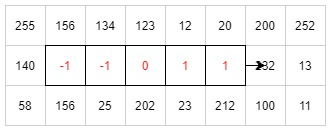
\includegraphics[scale = 0.4]{Method2Matrix.jpg}
            \centering
            \caption{1D Sobel kernel visualisation}
            \label{fig:InitalDesign}
\end{minipage}
\end{figure}

\textbf{Horizontal camera orientation and highlighting}

Due to the operation of the horizontal Sobel filter it detects vertical edge in the image, This is because it is moving through the image horizontally and highlighting an edge that may occur in its horizontal buffer which is always a vertical edge in the image. However in our analysis we are only interested in horizontal edges. So a simple solution  is to rotate the camera 90$^\circ$. thus the buffer now moves through the image vertically (respective to the video) and highlights horizontal edges as we desire.

\textbf{Analysis of highlighted edge video stream}

We then analyse the edge video stream in the following way : First the height of the image was divided into  80 vertical sections, each section has a sum and count which is reset when we enter a new section. When a white pixel is defected in this vertical section we add the vertical position of the white pixel to the sum and increment the count. At the end of the section we divide the sum by the count then inputting this result into the memory array for communication to the Command subsystem. When the final section is complete we reset the sum and count for the next frame. This process is done for only part of the image excluding data at the top of the camera as it is visually too far from the rover. 

\subsubsection{Communication to control subsystem:}

To communicate with the arduino we are connected via 3 GPIO pins which we use to implement a basic SPI communication protocol  . The pins are select , MISO and clkArduino . when select is low the arduino begins to request data from the FPGA when select is high is is not requesting. The miso line is the avenue which the bit stream of data from the memory array will flow. The memory array is a bank 98 registers storing 1 byte each. The first memory register is loaded with an open message symbol \verb|'{'| in ascii 123 and the 98th register is a close message symbol \verb|'}'| in ascii 125. The memory bank is read from 1 register at a time from start to finish where on each block pulse the next bit is read. With byte and bit addresses being updated for as we move through the registers. The implementation can be seen below and is relatively simple: 

\begin{figure}[hbt]
\begin{minipage}{.56\textwidth}
\begin{minted}[fontsize=\footnotesize]{verilog}
always @(posedge clkArduino) begin
if ( selectArduino == 0)begin
  miso  <= (counterByteAddress < 7'd100) 
  ? mem[counterByteAddress][counterBitAddress] : 0 ;
  counterBitAddress <= counterBitAddress + 3'b1 ;
  counterByteAddress <= counterByteAddress 
  + (counterBitAddress == 3'b111);
end    
if ( selectArduino == 1)begin
  miso <= 0 ;
  counterBitAddress <= 3'b0 ;
  counterByteAddress <= 7'b0;
end end
\end{minted}
\end{minipage}
\begin{minipage}{.43\textwidth}
        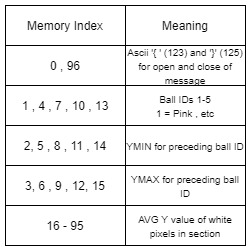
\includegraphics[scale = 0.4]{memoryMap.jpg}
            \centering
            \caption{Memory map}
            \label{fig:InitalDesign}
\end{minipage}
\end{figure}



\subsubsection{Ball detection Implementation:}

Each ball is detected using the same process using modified thresholds. The process begins by converting the RGB space into a highlighted HUE space representation. According to the HUE regions we assign either a white or black value to the pixel. For example, if the RGB values of the pixel lie in the orange HUE region we set the HUE\verb|_|Orange value to 0 for black. If it does not lie in this region we set it to 255 for white. This process is implemented as such:

\begin{figure}[hbt]
\begin{minipage}{.54\textwidth}
\begin{minted}[fontsize=\footnotesize]{verilog}
reg  [7:0]HUE_Orange ; 
always@(posedge clk) begin
if(R >= G)begin 
	if(R >=  B)begin  // R > G  && R > B, R IS MAX
		if (G >= B )begin // R MAX B MIN
			HUE_Orange <=  8'd0; 
		end 
		else begin // R MAX G MIN
			HUE_Orange <=  8'd255; 
		end
	end
end
//Implementation is cut here as too long but can be 
            //found in appendix
\end{minted}
\end{minipage}
\begin{minipage}{.45\textwidth}
            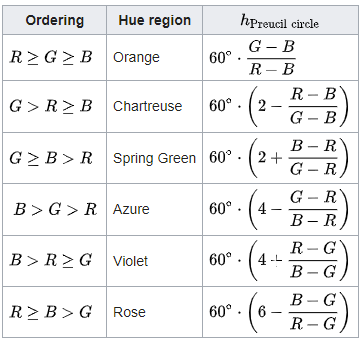
\includegraphics[scale = 0.4]{HueRegions.PNG}
            \centering
            \caption{HUE region table \cite{HueWikipedia}}
            \label{fig:InitalDesign}
\end{minipage}
\end{figure}

However some noise/unexpected RGB value exist which disrupts the bounding which occurs later. This to filter stray highlighted pixels that speckle across the image, we have a very simple filtering process. We use a buffer to store the current and previous 4 highlighted HUE values of the pixels (Using a buffer process shown below) . We then examine the top bit of this values, If its 0 then it will be highlighted and if its 1 its not, Thus if all stored pixel HUE values are 0 then all are highlighted and we accept this is not noise but a consistent region of orange/black/pink hue. As such we then re-highlight this pixel as white (Implying non noise) and black if it is noise. This leaves us with a image as such:

\begin{figure}[hbt]
\begin{minipage}{.49\textwidth}
\begin{minted}[fontsize=\footnotesize]{verilog}
wire  Orange_detect  ; 
assign Orange_detect = ~HUE_Orange_buffer[4][7] 
                    && ~HUE_Orange_buffer[3][7] 
                    && ~HUE_Orange_buffer[2][7] 
                    && ~HUE_Orange_buffer[1][7] 
                    && ~HUE_Orange_buffer[0][7]  ; 
wire [23:0] HUE_Out_Orange  ;
assign HUE_Out_Orange = {Orange_detect, ... ,Orange_detect} ; 

\end{minted}
\end{minipage}
\begin{minipage}{.49\textwidth}
            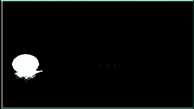
\includegraphics[scale = .8]{Detect.PNG}
            \centering
            \caption{Highlighted detected image (Orange)}
            \label{fig:InitalDesign}
\end{minipage}
\end{figure}

We now apply the simple bounding box process upon this filtered highlighted hue space The values of Ymin , Ymax and Xmin Xmax for each ball are updated at the eop for each frame. This method works relatively robustly but can be affected by high contrast conditions. As such we keep our camera in a low contrast / low brightness mode when bounding the boxes which seems is a preferable environment. 

\begin{figure}[hbt]
    \centering
    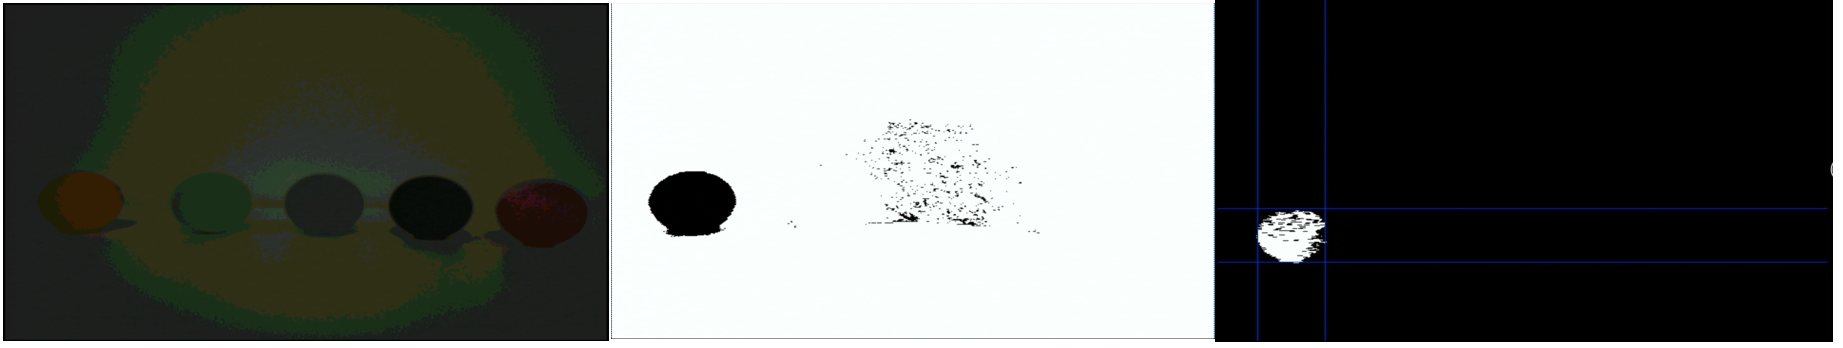
\includegraphics[scale = 0.25]{AnalysisImag.PNG}
    \caption{Highlighted Hue space before and after noise filtering}
    \label{fig:HightedHueSpace}
\end{figure}



\newpage
\newpage
\subsection{Command}
\subsubsection{Overview of Design}
The overall design of the command module has it split into two main components, the front end that the user interacts with in their browser and the back end that runs on a server in the cloud. The server is responsible for making all of the decisions for the rover as it can be given as much computing power as is needed, meaning more complex decisions can be taken quicker. The rover itself will send information about its change in polar coordinates after every movement it completes to the server, the server will then use the information it has to send a new movement to the rover. The user interface will concurrently request data from the server about the rover to present to the user, and will send user commands to the server to allow it to make movement decisions. 

The user interface allows for three different methods for controlling the rover. The first is the most simple and consists of sending direct commands, such as move forward x steps, turn x degrees or stop. When the rover is executing these commands it will not avoid any obstacles in its way. The second means of control is the sending of coordinates to the rover, this is done through the user clicking on a map of the rovers surrounding to give it a desired location, the rover will then move to this location avoiding any obstacles on the way. The final method of control allows the user to specify a ball that the rover should find. The rover will head to this ball if its location is known else it will search its surrounding until it does, in this mode as well as in the coordinate mode the rover will avoid obstacles and will automatically head back to the charging station if low on power. The flow diagram in figure \ref{fig:CommandOverview} demonstrates the process the command system uses to communicate with the rover.

The server was built using Python and used flask library for handling http request. This decision was made as Python has extensive libraries for mathematics meaning calculating the commands for the rover would be easier. The flask library was used as it is very light weight and doesn't come with loads of extra features that we wouldn't need to use. The user interface was made using flutter, this allowed the app to be compiled as either a desktop app or as a website without changing any code. The python server and the static files for the interface were deployed on the Digital Ocean App Platform. This means of deployment was chosen as it is extremely user friendly speeding up development time and deals with services such as SSL certificates automatically.

\begin{figure}[hbt]
    \centering
    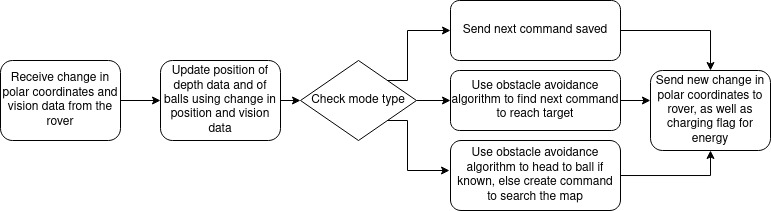
\includegraphics[scale = 0.6]{CommandOverview.jpg}
    \caption{Top level overview of the command system}
    \label{fig:CommandOverview}
\end{figure}

\subsubsection{Receiving data to and from the rover}
The data received from the rover is in the form of a Json file. These Json files used for each communication direction have a schema that was carefully designed with the control system so as to ensure that both systems could be worked on independently as the input and outputs between each system were well defined. The schemas themselves went under many revisions as the design was changed over time. The rover itself communicated with the server using a single POST request, whilst the user interface communicated using many different GET and POST requests. The interface would continuously poll the server for new information to always stay up to date.

\subsubsection{Updating Map Information}
Once a movement was received from the rover the servers current knowledge of the map needed to be updated using this new information. The two main changes that needed to be made were updates to depth information and to ball information, as well as to the target location.

\subsubsection{Updating Ball Information}

The position of any balls know to the server were stored in polar coordinates. These coordinates would always be relative to the rovers forward direction. This meant that the first step in updating their position to was to convert their positions to Cartesian coordinates. Then the polar changes received from control for the last movement could also be converting to Cartesian and the resulting $dx$ and $dy$ be applied to the ball positions, before finally converting back to polar. These new polar coordinates would also have to be rotated in order to be with respect to the new forward direction of the rover. All polar angles were taken from the clockwise forward direction of the rover. The block diagram for this logic is shown in figure \ref{fig:CommandBallPosition}. In order to test this logic in python the library "matplotlib" was used. This meant that the balls could easily be plotted before and after a movement in order to see that the resultant change in position is the expected one. The decision to use polar coordinates for storage was used as it makes it more intuitive to imagine the change in the rovers axis as it is simpler to imagine rotations, it is also closer to the manner in which the balls are perceived by the rover. 

\begin{figure}[hbt]
    \centering
    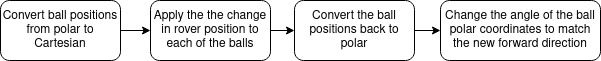
\includegraphics[scale = 0.6]{CommandBallPosition.jpg}
    \caption{Overview of the ball position updating}
    \label{fig:CommandBallPosition}
\end{figure}

Once all the positions of know balls is updated the position of any new balls has to be added. The information the rover receives about new balls is in the form to of two values from the vision system. These two values represent the horizontal camera position of the two sides of the balls in the camera view. From these two values the polar angle of the centre of the ball horizontally can be calculated. This requires imagining how the flat view of the camera is projected onto a curved view and can be done using the equation below. The angle $\alpha$ is the desired angle. The diagram is shown from which these equations were created, the point $C$ represents the midpoint between the the two given points $A$ and $B$, the value $l$ can be treated as one as it is cancelled when evaluating the final equation.
\begin{minipage}{.5\textwidth}
\begin{gather}
\frac{l}{2r}=sin(\gamma/2) \\
r = \frac{l}{2sin(\gamma/2} \\
x = \sqrt{r^2 + c^2 - 2rccos(90-\gamma/2)} \\
\alpha = sin^{-1}(\frac{c*sin(90-\gamma/2}{x})
\end{gather}
\end{minipage}
\begin{minipage}{.5\textwidth}
    \centering
    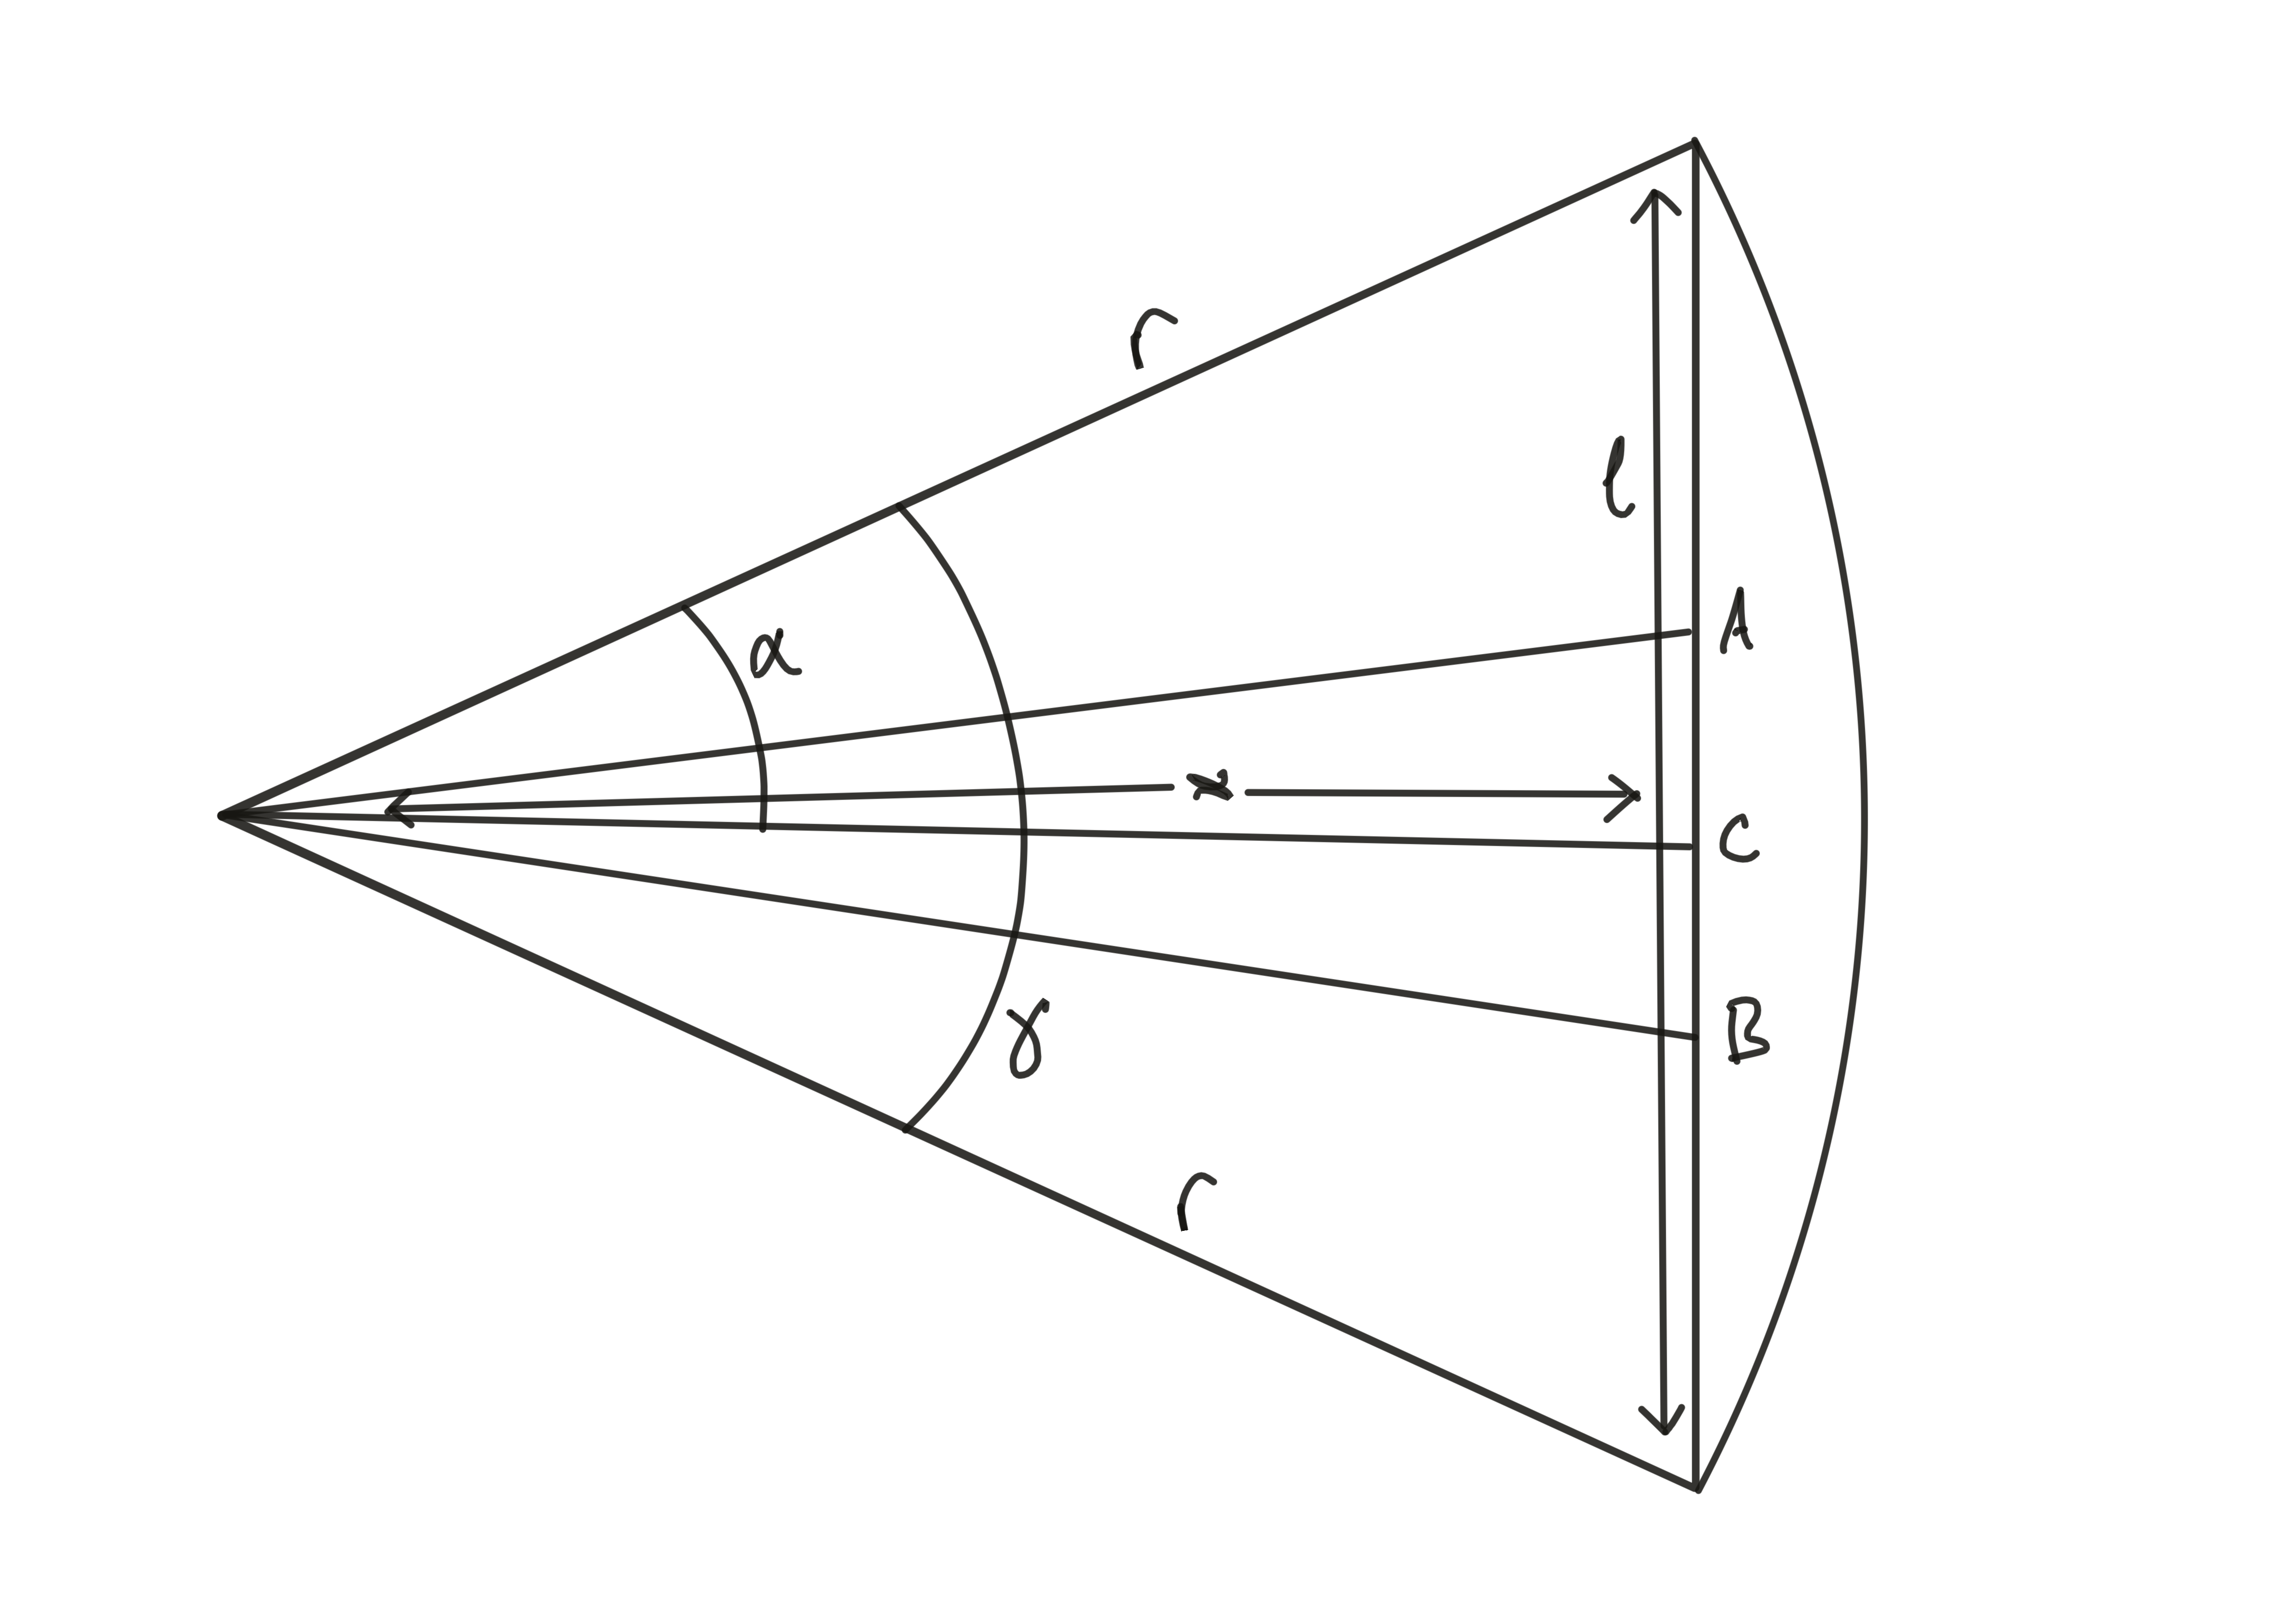
\includegraphics[scale = 0.6]{CommandFOV.png}
    \caption{Camera field of view diagram}
    \label{fig:CommandFOV}
\end{minipage}
\\
Once this angle is calculated the distance to the ball can be calculated using the distance between the two values as the diameter of the ball is known. This is achieved using the equation below. Once the coordinates of any new balls is found they are added to the map and replace their old position if they had been previously detected. The angle $\beta$ used is the angle between the two detected edges calculated using the value $\alpha$ from above. The value $d$ is the diameter of one of the balls and $D$ is the distance to the ball.
\begin{gather}
D = \frac{d}{2tan(\beta/2}
\end{gather}

\subsubsection{Updating Depth Information}
Once the position of the balls had been calculated an estimation of the depth to any object not just including balls was calculated. An algorithm was developed for this separately as a proof of concept before beginning work on the rover implementation. The basic idea is that it should be possible to detect the distance towards objects using two different images taken at different positions. The first step to be able to do this was to apply an edge detection algorithm to the image. This was done in testing using the python "Open CV" library. The algorithm we then used for to detect depth on this image was very simple. The principal is that horizontal edges that are closer to the rover will move more between frames than edges that are further from the user. Therefore, the average position of all the white pixels in every vertical row of the image is calculated to measure this change. Another image is then needed taken closer to the object, this was done in testing using a video from a mobile phone using every $20th$ frame. The percentage change of the average position of any white pixels within a vertical row is then taken and this is used as the distance estimator. This method is inspired from an extremely simplified version of optical flow, which is used to detect movement in images. The results from testing can be shown plotted with the image in figure \ref{fig:CommandUnfilteredVision}. The edge detection version of the photo is shown in figure \ref{fig:Commandbottles}, the photo is of two bottles placed at different distances.

\begin{figure}[hbt]
    \centering
    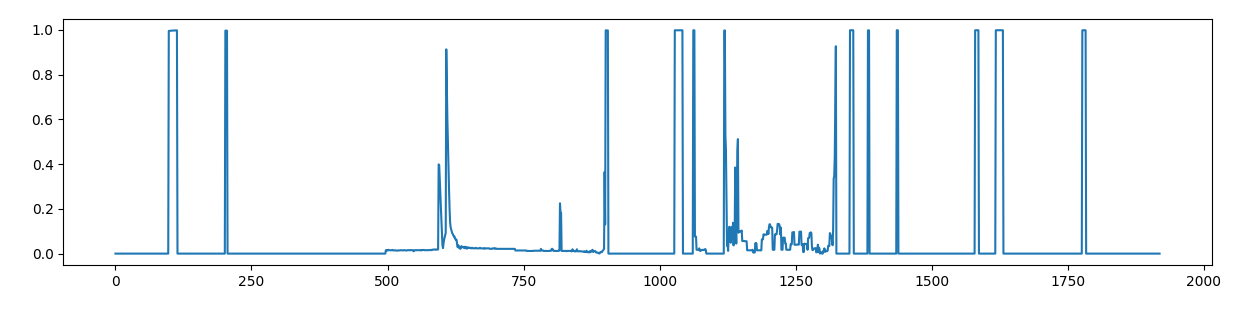
\includegraphics[scale = 0.4]{Commandunfilteredvision.png}
    \caption{Unfiltered algorithm output}
    \label{fig:CommandUnfilteredVision}
\end{figure}


\begin{figure}[hbt]
    \centering
    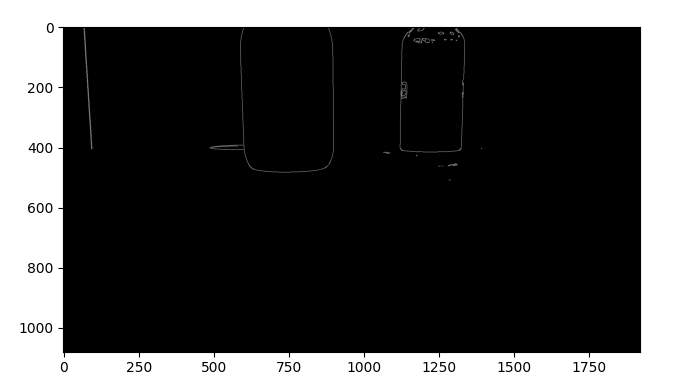
\includegraphics[scale = 0.6]{Commandbottles.png}
    \caption{Edge detection on image of two bottles}
    \label{fig:Commandbottles}
\end{figure}

Since this this data is very noisy a moving average filter was taken over the data. This still resulted in several small spikes, and so any spikes that were below a certain width were then removed from the data. This was done by checking each window of the data and seeing the maximum change and maximum fall. If the fall and gain were both over a threshold all the data in the window was set to the minimum of the window. The results from testing using this methodology can be seen in figure \ref{fig:CommandFilteredDepth}. As can be see this does give a good estimator of depth and can certainly be used to notify a user if an object is within the path of the rover. The flow chart for this diagram is shown in figure \ref{fig:CommandDepthFlow}. This was decided to be a good enough proof of concept and so the algorithm was incorporated into the server code with data coming from the rover itself. The server uses data sent after every movement and only uses the new data if it has not changed orientation. 

\begin{figure}[hbt]
    \centering
    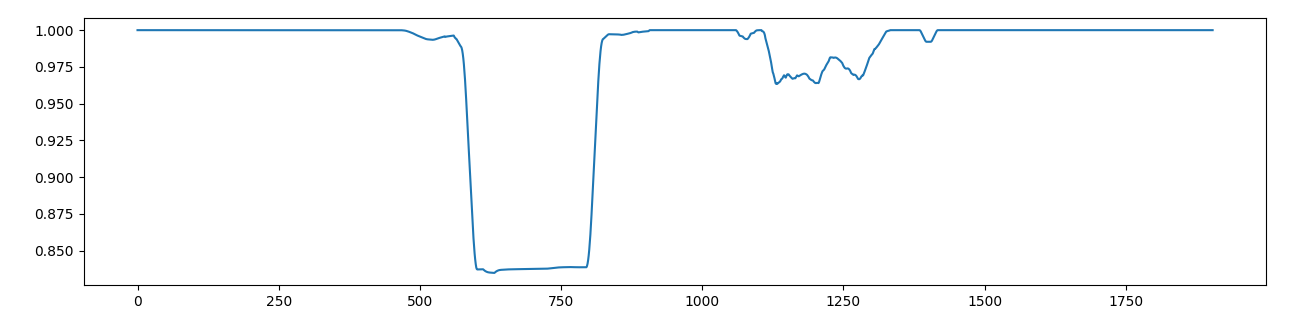
\includegraphics[scale = 0.4]{CommandFiltered.png}
    \caption{Filtered algorithm output}
    \label{fig:CommandFilteredDepth}
\end{figure}


\begin{figure}[hbt]
    \centering
    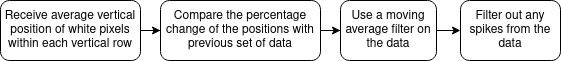
\includegraphics[scale = 0.6]{CommandDepthFlow.png}
    \caption{Flow diagram for depth detection algorithm}
    \label{fig:CommandDepthFlow}
\end{figure}

Initially when depth data had been calculated we wanted to have it be remembered if the rover was to turn around, giving a full 360 estimator of depth at all times. In order to accomplish this the depth data was stored in an array, with its index representing its angle and its value representing depth, and after every movement was updated similarly to how the ball data was updated. Firstly, every point had its position converted to Cartesian and was translated by the rover movement. Then each point was converted back to polar coordinates. The data however was needed at specific angles corresponding to indexes of the array and so the the average depth of the data either side of the desired angle was taken. After this the data was rotated to represent the change in rover orientation. This could then be sent to the user interface and plotted on the map as shown be the circle. We found however that the depth data was to inaccurate to bother with this method and so only the arc representing the rovers current field of view was used so no data had to be translated. As with the balls, whilst developing this "matplotlib" was used to visualise the translation of the coordinates.

\subsubsection{Deciding Next Move}
In order to decide upon the next move for the rover the server first checks the current movement mode type and then call one of three functions in order to create the move, the three movement modes are command, search and map.

\subsubsection{Command Move}
Creating a command move is the simplest mode. The three types of command the rover can receive are "forward(x)" where x is the distance in mm, "turn(y)" where y is the angle in degrees to turn and finally "stop", which clear all saved and in progress commands. Commands are sent by the user through the user interface to the server and are kept in a stack object and cleared as they are executed. Since the rover only computes small movements before checking in with the vision section any command that requires a movement or turn greater than the maximum movement or turn is broken up into sub commands that add up to the movement. This means that when the rover requests a movement the server first checks if a sub command exists, if it does it takes it from the sub command stack and sends it to the rover, if it doesn't it takes the next main command splits it into sub-commands which are added to the sub command stack. The first sub command is then sent. If the server receives a stop command from the user all sub commands and main commands are deleted.

\subsubsection{Map Move}
In map mode the user sends a coordinate to the rover that it should complete, a movement command therefore  needs to take the user closer to the required target. Firstly, the rover checks if it is low on charge relative to the distance to the charging station, if it is it uses that as the target otherwise it uses the user coordinate as the target. In initial testing the server would just send then target straight to the drive system and the drive would only complete the maximum allowed distance. An obstacle avoidance system was then created to find the optimum path to the target avoiding any balls on the way.

\subsubsection{Obstacle avoidance}
In order to make the Rover fully autonomous a general obstacle avoidance algorithm was developed. This allows the Rover to reach a given destination whilst making intelligent decisions on how to avoid obstacles on the way.
The algorithm works in the following way:
\begin{itemize}
    \item Receive information of the obstacles nearby from the sensors
    \item Construct a graph with the sensors' information. The graph represents a "map" of the surroundings. Every node on the graph represents a location where the rover is allowed to move. Nodes are removed form the graph where an obstacle is present. A fixed weight of one is assigned to the edge connecting a node to any of its neighbors.
    \item An algorithm to find the shortest weighted path between the location of the rover and the destination is applied.
    \item As the Rover moves towards the destination, the "map" is updated with new obstacle information. The shortest weighted path to the destination is recomputed and the Rovers changes direction accordingly
\end{itemize}

\textbf{Best path algorithm} Dijkstra's algorithm was used to find the shortest path between two points in the "map". This was later on improved and transformed in a A* algorithm by adding a heuristic function to give priority to nodes closer to the destination. The code for these implementations was adapted from \cite{AWikipedia},\cite{AAB} and \cite{ImplementationA}.



\subsubsection{Search Move}
In  search mode the rover is given specific ball colour to go towards, if the balls position is unknown the rover must search the surroundings for it. Designing the route the rover should take to search the map was the core part of a this mode. It was decided that no particular direction should be prioritised over any other and for this reason a spiral route was chosen, with the center being the charging station. This was chosen as it allows the rover to view the map from many angles and always covers ground closer to the rover before ground further away. Since the distance between spiral turn should remain constant an Archimedes's spiral was used as it has this property. The equation is shown below,
$$
r = a\theta
$$
and simply makes the radius of rotation in direct proportion to the total angle change. Using this equation it is necessary to calculate the movement the rover should take given that it is a given distance from the charging station and is facing 90 degrees to it. The diagram and equations show how to calculate this polar coordinate relative to the rover, the distance $x$ here is the desired depth the rover should move forward and $r$ is the distance to the charging station.
\begin{minipage}{.5\textwidth}
\begin{gather}
\frac{l}{2r}=sin(\gamma/2) \\
\frac{x}{sin(\gamma} = \frac{r+a\gamma}{sin(\beta} \\
\beta = sin^{-1}((r+a\gamma)*sin(\gamm))
\end{gather}
\end{minipage}
\begin{minipage}{.5\textwidth}
    \centering
    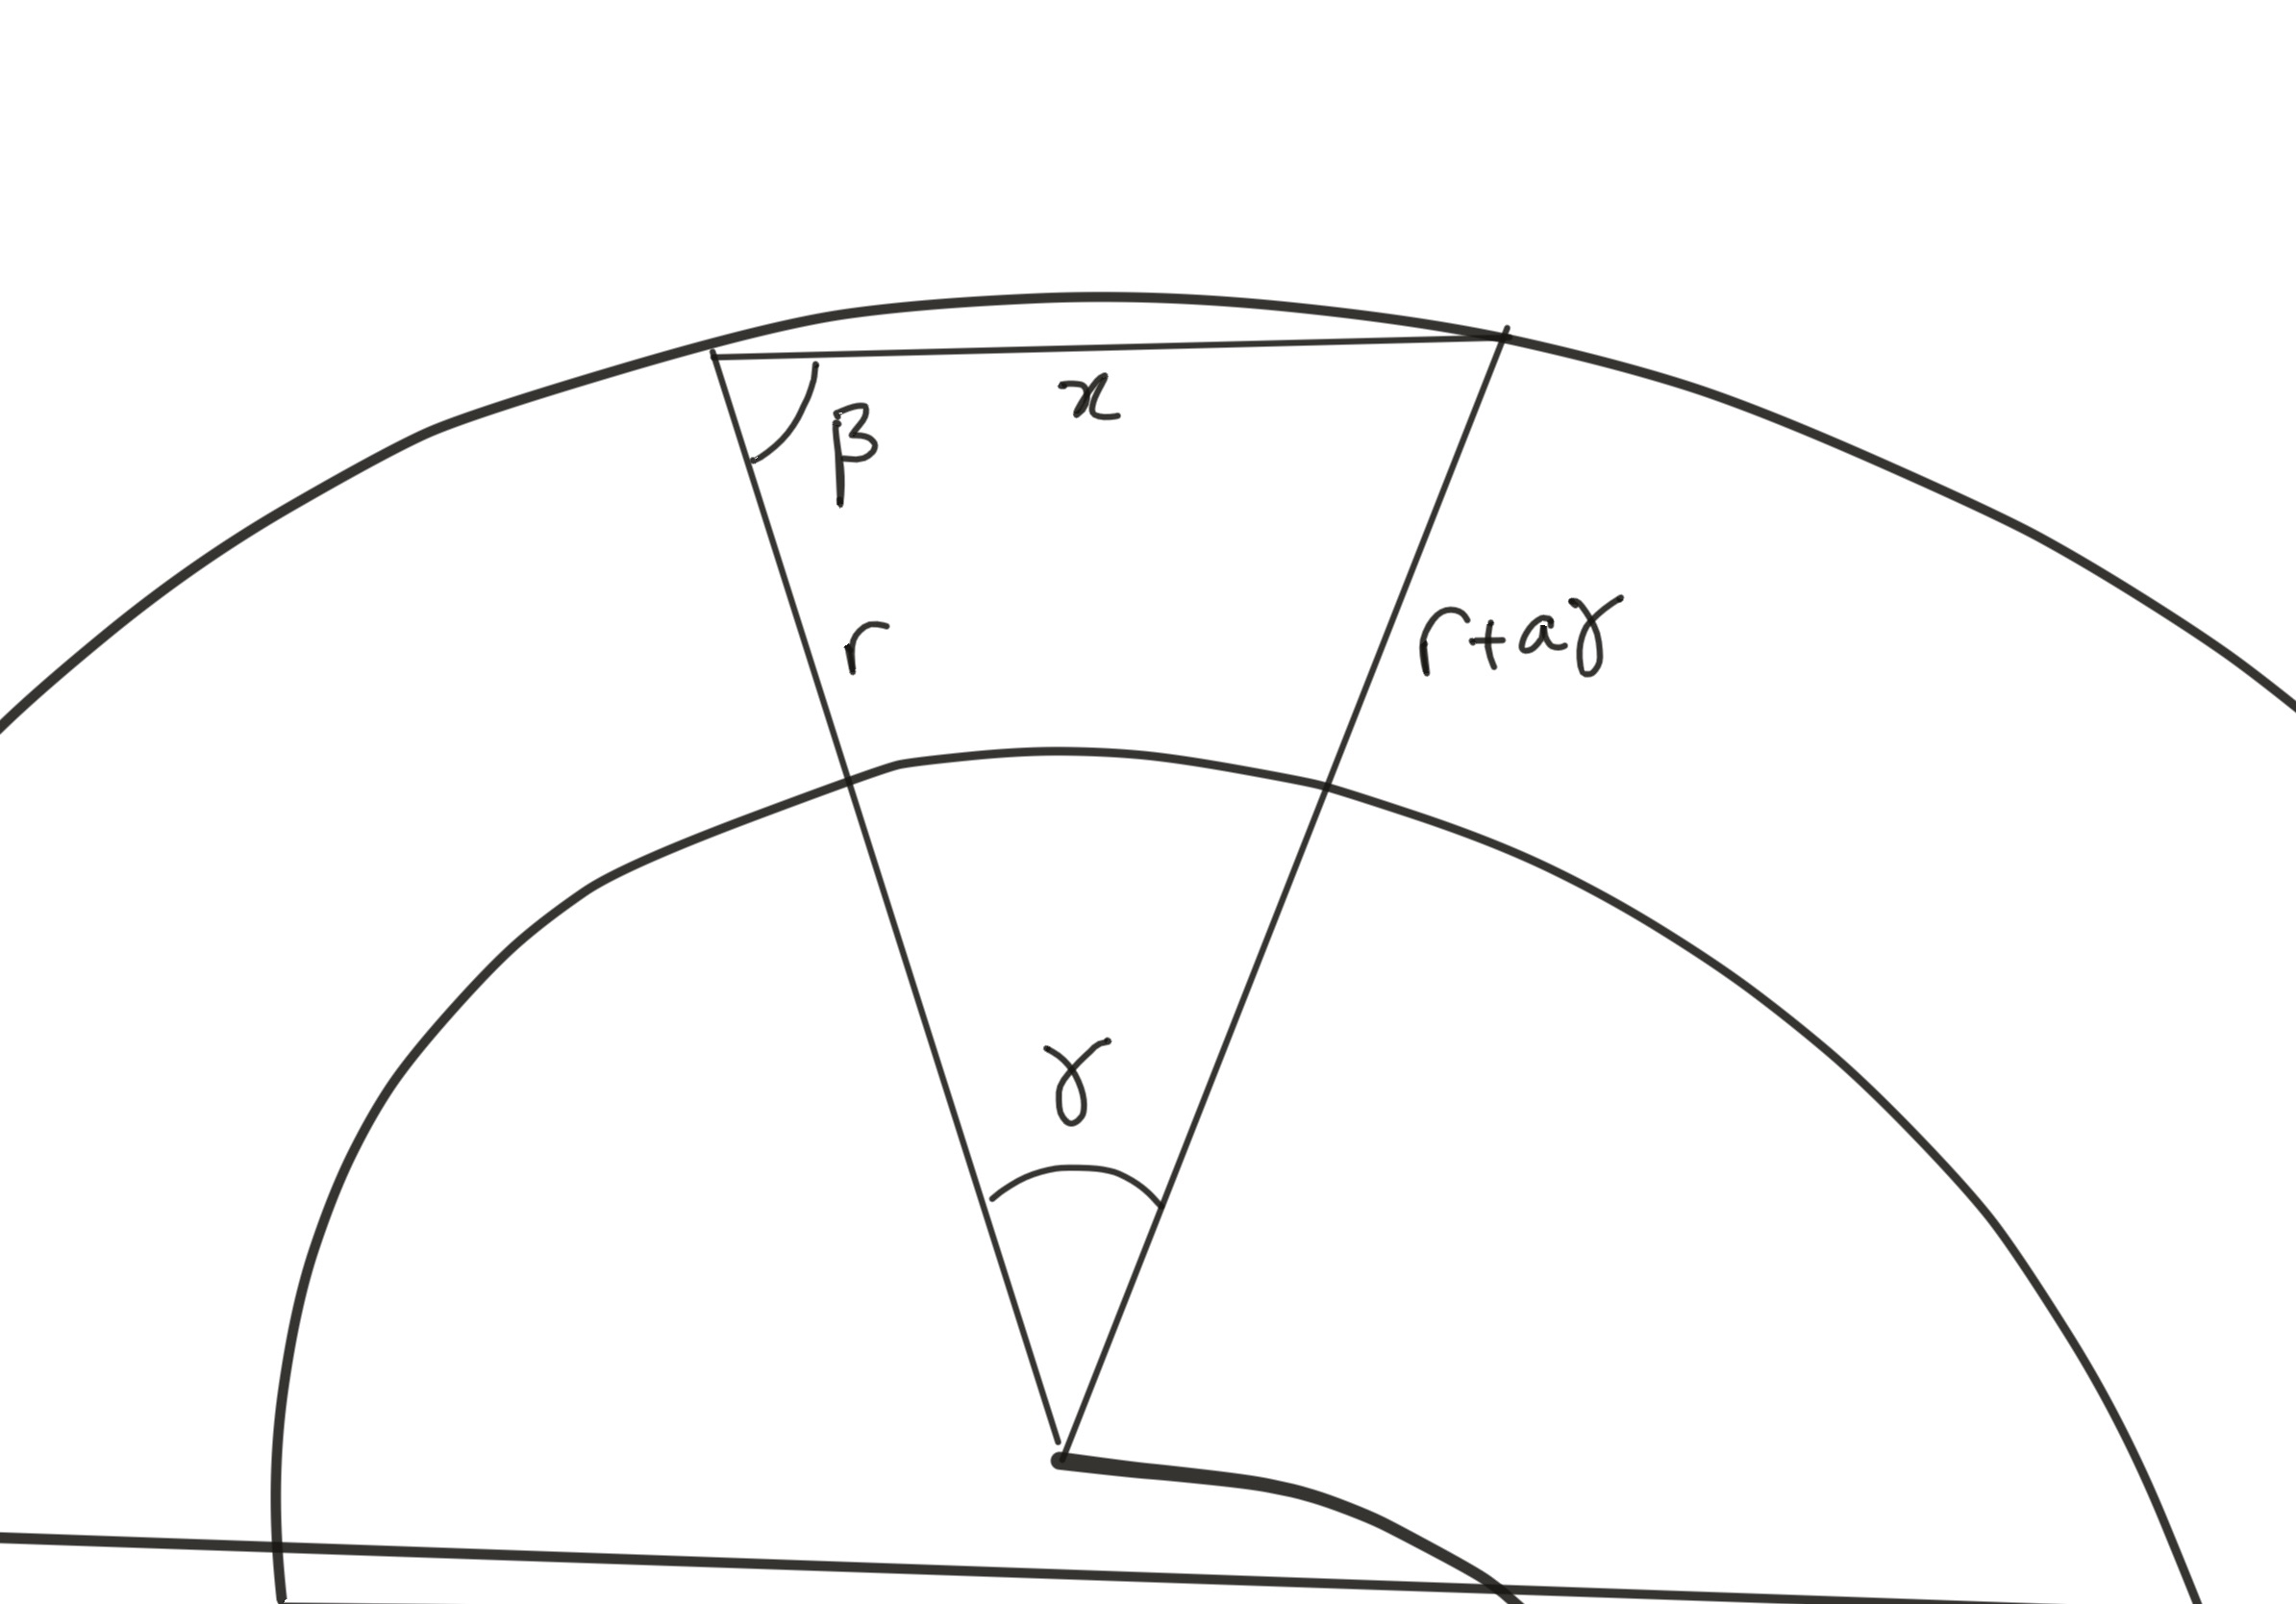
\includegraphics[scale = 0.1]{CommandSpiral.jpg}
    \caption{Diagram of position change for spiral movement}
    \label{fig:CommandFOV}
\end{minipage}
This equation was tested using "matplotlib" and gave good results. It was found however in testing that the following code gave very similar results and is much less computationally expensive and so was used instead giving the results shown in figure \ref{fig:CommandSpiralView}. 
\begin{minted}[fontsize=\footnotesize]{python}
angle = angle_to_charge + 90 //angle that the rover should turn should be 90 degrees to the charging station
angle %= 360
theta = 0.7 - pow(math.e, -1 * distance / 100) * 0.7 //this value is used to keep the distance between spiral turns constant
angle += theta
angle = angle % 360
\end{minted}
Once this coordinate is given it is then treated as a target for the map mode command creation with employs the obstacle avoidance meaning the rover will avoid any other balls it meets on the way. If the rover finds it is low on charge relative to the distance from the charging station it will head back to the charging station. The rover will then head back to the radius it was at previously. The flow diagram for the search mode algorithm is shown in figure \ref{fig:SpiralMoveFlow}.

\begin{minipage}{.5\textwidth}
    \centering
    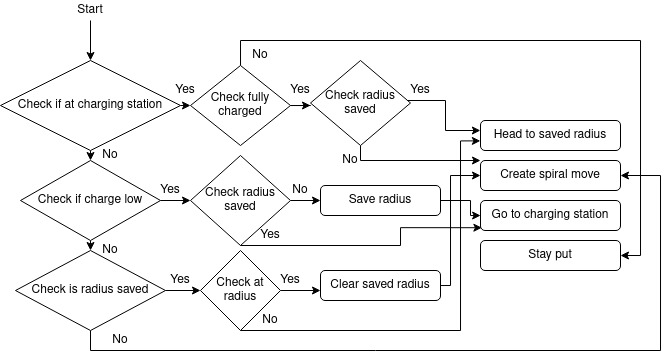
\includegraphics[scale = 0.7]{CommandSpiralMoveFlowAlgo.jpg}
    \caption{Flow diagram for spiral move algorithm}
    \label{fig:SpiralMoveFlow}
\end{minipage}

\begin{figure}[hbt]
    \centering
    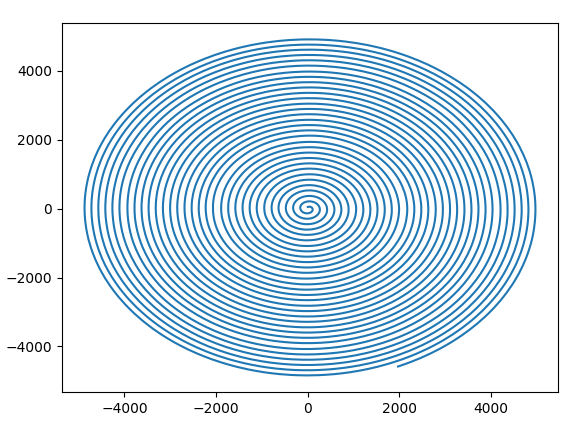
\includegraphics[scale = 0.4]{CommandSpiralView.png}
    \caption{A simulated plot of the spiral movements of the rover}
    \label{fig:CommandSpiralView}
\end{figure}

\subsubsection{Design of The user Interface}
The user interface was built using the flutter toolkit from google. This meant that a cross platform app could be easily built that could run as a desktop app or in a browser providing more options to the users. The app was designed to present all the information to the user at once, avoiding pagination so that commands can be made as quick as possible. The photos in the appendix show the design of the interface. A panel on the right changes depending on the command mode the user selects. It either shows coordinates of targets and balls for the map mode, a command input and list of commands for command mode or the option to select which ball to search for in search mode. On the left the interface shows a map that indicates the position of any balls relative to the rover and can also display the depth information. The user can also click on this map to select the target coordinate for the rover. Finally along the bottom information such as battery charge and health is displayed along with a speed control option for the rover.




\subsection{Control}


\subsubsection{Message protocol} 
In order to communicate with the Drive, Vision and Energy subsystems a general message protocol has been designed to ensure that only valid data is received. The message is composed by:
\begin{itemize}[noitemsep]
    \item Start of Message (SOM) character, used to identify the beginning of the message.
    \item The payload of the message. The size and structure of the payload is fixed and depends on the specific subsystem considered.
    \item an End of Message (EOM) character, used to identify the end of the message.
\end{itemize}

Messages are constructed and sent byte by byte according to the protocol specified above.
The transmitter sends a message in the following way:
\begin{itemize}[noitemsep]
    \item Send SOM.
    \item Send the payload. Each subsystem expects data (characters) to be in a specific order. It is important that this predefined order is respected to communicate successfully. 
    \item Send EOM.
\end{itemize}
This ensures that the receiver can safely receive a message by:
\begin{itemize}[noitemsep]
    \item Wait until Start of Message character is received.
    \item Receive the payload of the message.
    \item Stop receiving when the End of Message character is encountered.
\end{itemize}

The diagram in Figure \ref{fig:SendAndReceive} shows how data is sent and received.

\begin{figure}[hbt]
    \centering
    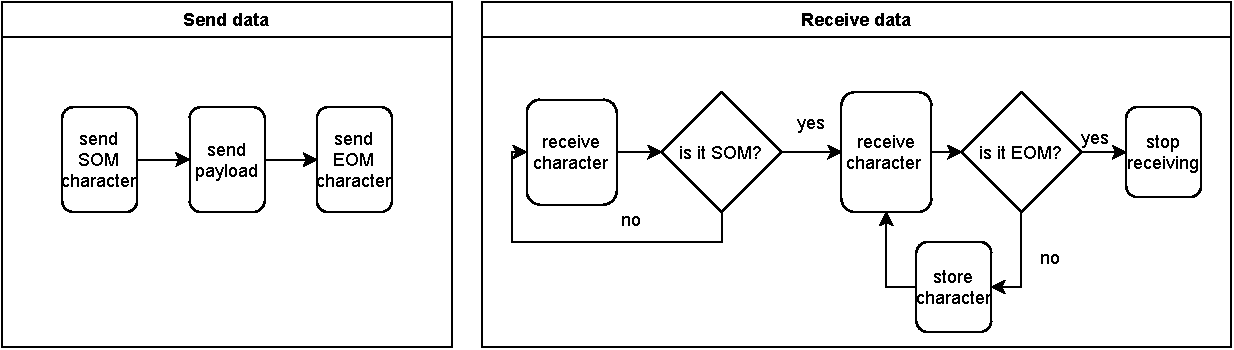
\includegraphics[width = \textwidth]{Send_and_receive.pdf}
    \caption{Sending and Receiving data}
    \label{fig:SendAndReceive}
\end{figure}


\subsubsection{Data Timing} 
The ESP32 is what controls and manages the flow of information. It collects data from every subsystem, sends it to the server for processing and finally receives back data to reach the next destination.


\paragraph{Independent communication with each subsystem:}
Priority was given to implementing communication between Control and each single subsystem. A suitable message protocol was designed according to the data exchanged with each subsystem. Tests were carried out making sure that the data sent from one subsystem matched with the data received by the other subsystem.

\paragraph{General communication between subsystems $\vert$ Version 1}
The next step was designing the general data flow between every subsystem. JSON  documents were chosen as  our  file  format  for  data  interchange because:
\begin{itemize}
    \item JSON documents provide an easy way of merging the data collected from each subsystem in a single file
    \item There are well documented libraries for ESP32 that make the serialization/de-serialization process easy for the Control subsystem and the Command subsystem
\end{itemize}
The data flow is \textbf{sequential} and data is received in order from Drive, Energy and Vision. A JSON document is constructed with the collected data and sent to Command. Finally the response form Command is sent to Drive.

\paragraph{General communication between subsystems $\vert$ Version 2}
Our design specification required fast bidirectional communication between Energy and Control. This has been the biggest challenge in the implementation of the Control subsystem. The Energy arduino code would not function correctly if delays due to receiving data are introduced. The source of this delay are the computations performed on the server and the inherent single delays due to the sequential communication with every other subsystem. The solution that we adopted for this problem was \textbf{parallel} communication.
This was achieved by exploiting  the dual-core nature of the ESP32. In particular the communication flow was split between the two cores in the following way: 
\begin{itemize}
    \item \emph{Core1} manages receiving data from Drive, Energy and Vision. It also manages communication with the server and forwards data to the Drive subsystem to compute the next move
    \item \emph{Core2} continuously sends data to Energy. This ensures that new data is always ready to be received and hence there are no delays from the point of view of the energy subsystem due to to communication
\end{itemize}

The flow of information is described in Figure \ref{fig:DataFlowDualCore}.#



\begin{figure}[hbt!]
    \centering
    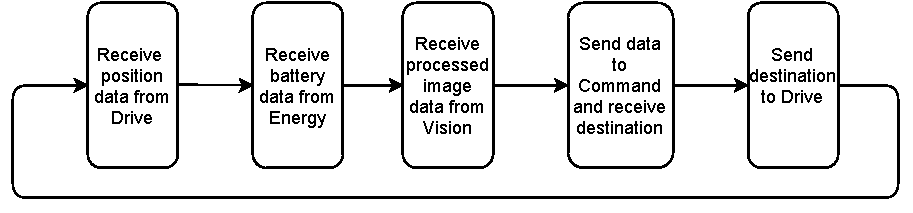
\includegraphics[scale=0.5]{esp32_flowchart.pdf}
    \captionsetup{justification=centering}
    \caption{High Level data flow}
    \label{fig:DataFlowDualCore}
\end{figure}


\subsubsection{Communication protocols} 
Suitable communication protocols have been chosen in order to meet the design criteria.
For each communication protocol speed of communication, reliability, direction of communication and hardware availability were analyzed for a given subsystem. Whenever multiple communication protocols satisfied the design criteria, the simplest option to implement was selected.


\paragraph{UART} The UART communication protocol has been chosen for data transmission between Drive and Control and between Energy and Control. 
In particular UART was chosen because: 
\begin{itemize}[noitemsep]
    \item It is fast enough for the application: the Drive and Energy subsystem only need to exchange small amounts of data (small payload size)
    \item It has in-built error detection and correction
    \item It allows full-duplex communication. Full-duplex is essential for Control-Energy communication as it allows receiving and sending data at the same time
    \item It is easier to implement than SPI
\end{itemize}


\paragraph{SPI} The SPI communication protocol has been chosen for data transmission between Vision and Control.
In particular SPI was chosen because: 
\begin{itemize}[noitemsep]
    \item It allows for high speed data transmission and is faster than UART or I2C. This makes it suitable for transmitting large amount of data such as image data received from Vision  (large payload size)
    \item It provides robust error detection features
\end{itemize}


\paragraph{WiFi and HTTP} The Rover communicates with the remote server using WiFi.
WiFi was chosen over Bluetooth because:
\begin{itemize}[noitemsep]
    \item WiFi range is much bigger than Bluetooth range. This means that the rover can explore a wider area of the Mars surface whilst still communicating with the Server
    \item WiFi provides better wireless security than Bluetooth making unauthorized accesses to the server harder
    \item WiFi connection is faster than Bluetooth. This allows efficient data exchange between the Rover and the Server
\end{itemize}

Data is exchanged between Control and Command using HTTPS POST requests. HTTPS was chosen over other standards because:
\begin{itemize}[noitemsep]
    \item It is fast enough for the application: it satisfies the speed design criteria standards
    \item It provides enhanced security by encrypting the data exchanged
    \item It is compatible with the JSON documents library used on the ESP32.
\end{itemize}
 

\begin{figure}[hbt!]
    \centering
    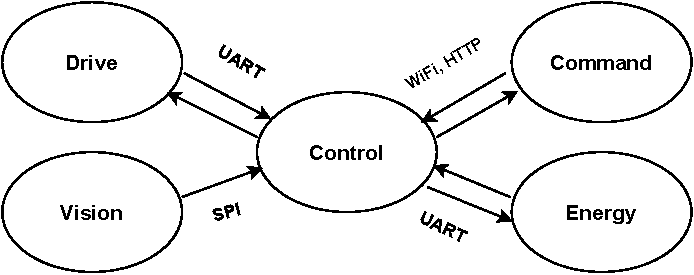
\includegraphics[scale=0.7]{Communication_protocols.pdf}
    \captionsetup{justification=centering}
    \caption{Communication Protocols}
\end{figure}

\newpage


\section{Testing and Evaluation}


\subsection{Drive}

The tests of the drive subsystem conducted throughout the project were of the following type:

\textbf{Functional testing}
\begin{enumerate}
    \item \textbf{Testing of the single parts of the subsystem:}
    \begin{enumerate}
        \item motor functionality:  turning, move forward and backwards where tested by hard-coding the distance and angle targets. Once overcome the problem represented by the cables obstructing the movements and the wheels getting stuck because of lose connections, the motors were found to be accurate in the movements even at maximum speed (for error calculation see testing of performance).
        \item SMPS functionality: a first delay was perceived when turning on the SMPS, this was fixed by setting the Buck to closed-loop mode and since a delay of 5seconds was still perceived because of the large capacitors used, this was later fixed by making the logic of the state machine idle for the first 5sec the SMSP is on (only the first time of the loop). Additionally, even though the SMPS was thought to received 6.4V at its input from the energy subsystem, this was not possible to be tested (battery problem), so just 5V were used at the input (standard power socket), giving an output voltage smaller or equal to 5V
        \item optical sensor functionality: the sensor was tested on different surfaces and its data checked via the Serial Monitor of the Arduino. The quality of the images (expressed in terms of stars) was so compromised with certain surfaces that would ruin the whole functionality and this was solved by creating the alternative, time-based model. However, in the right environment, the optical sensor was observed to be very precise and to represent the best available way of tracking the movements.
    \end{enumerate}	
    \item \textbf{Testing of the models:}
    
     The code for each component of drive subsystem was merged creating an auxiliary functions’ file in the same Arduino sketch to ease the reading of the main program; the data from the optical sensor was decided to be use for a feedback that would calculate the remaining path to be computed. Then, the functionality of each section was re-checked through the Serial Monitor and by inspection, confirming that the sensor and motors were working correctly and that the state machine of the moving algorithm would not lead to undefined states.
    For each further feature added to the main code, a series of functional testing were conducted to check both the original functionality and the expected behaviour from the addition. 
    Tests were made to check that the PID controller and the variable speed of the wheels were implemented correctly, before adding them to the code. It was measured that the minimum speed to be input at which the rover would start moving is above 5 rpm, with a maximum of 60rpm for the highest duty cycle (Vref of approximately 5V). Having found some bugs in the built-in PID controller provided in the relevant Arduino library, it was decided to create our own controller, which was tested with various input and then integrated to adjust the current speed (when moving forward) and speed difference of the wheels (when turning whilst moving).
\end{enumerate}
\textbf{Testing on the performance }

(These tests were done on the fully integrated rover since its weight and specific characteristics could influence the actual speed and precision of movements)
\begin{enumerate}
    \item \textbf{Arch trajectory model:} Following some research on the best optimal path to be computed by the rover to reach a give location, an alternative method for the movements was tested. This implied using an arch trajectory. However, some successful tests highlighted how this way did not enhanced the performance of the rover (neither in terms of speed, nor precision), whilst involving some extremely complicated calculations for the movements’ tracking. Therefore this model was discarded and the optimal path was then decided to be computed on the server side, which would send small, constantly updated instructions.
	\item \textbf{Optical sensor-based model:} This version was extensively verified to make sure both the turning and moving forward could be within the error stated in the requirements (10\%). Various paths and different sequence of commands were tested, and the result were the following: for flat non-homogeneous and non-reflective surfaces (e.g. wood) the precision of the movement was measured to be above 90\% , an extremely good results given the limitations of the sensor and the imperfections of the motors. The maximum errors measured for the distance and the angle were respectively of approximately 5mm and 5°. However, for other surfaces (e.g. white table or carpet) the optical sensor did not provide reliable data to be used in the feedback system.
	\item \textbf{Time-based model:} this back-up model was tested especially on the surfaces in which the optical sensor could not be used. The general results on the precision were overall satisfactory, with an error within 13%, as expected lower than the optical sensor model because of the lack of a feedback system.
	\item \textbf{Optical sensor-based model with PI controller:} this model was around the same level of precision in the movements as the one without a PI controller (within 10\% error), but the overall time spent before reaching the target was lower than the other one since the controller would decrease the speed when approaching the target, instead of since using constant maximum speed. This would have been an important feature if using high speed; however, an analysis of the performance showed how, in our case, the benefit of a speed control system did not increase the overall quality of the movements, since the other model would already compute well-controlled movements and did not produce a relevant overshoot, given that the distances and speed are always contained. Therefore, the model without PI controller was chosen for the final version.
\end{enumerate}
\textbf{Testing with the control and command unit}

For each model, the communication with the control unit was tested making sure the data sent and received was correct and that the functionality of the rover was not compromised. The delay measured between the end of the current instructions and the beginning of the next execution was measured to be??? below 0.5 sec??, meaning that the communication is fast enough to not cause a major delay between movements and allowing the instruction to be rather short but frequently updated. Various tests were conducted to check that the current location computed from the optical sensor coordinates was correctly updated on the monitor of the website and that the next instruction was calculated without errors.

\subsection{Energy}

\subsubsection{Cell Testing}

Testing Energy involved making a variety of programs which confirmed the performance of functions and helped in the further development of others. Figure \ref{fig:TestCCCV} was used to test the CCCV charging mode. It clearly worked well with the CV mode keeping the cell voltage at 3.6V and the charge ceasing when the current hit 50mA. This was then tested using the solar panels. The effect was less pronounced as the max lamp current is 70mA and therefore the 50mA limit was decreased to 20mA (Figure \ref{fig:CCCVPV}). However It was good to know that the voltage PID worked well in combination with the MPPT function (Note the fluctuating current). The SOC estimation was tested by having a discharge program which changed the current at 50\% as seen in figure \ref{fig:TestSOC}. The SOC was a linear line and steeper when -250mA was being discharged. It was expected that the line would be linear due to the constant current output and a change to a shallower gradient during the -125mA confirmed that the function was working as expected. The 2.6\% overshoot seems acceptable given that this was a first cycle with no SOH calibration. This also justifies the use of a 3\% tolerance with the balancing function.  

\begin{figure}[hbt!]
  \begin{minipage}[b]{0.47\textwidth}
    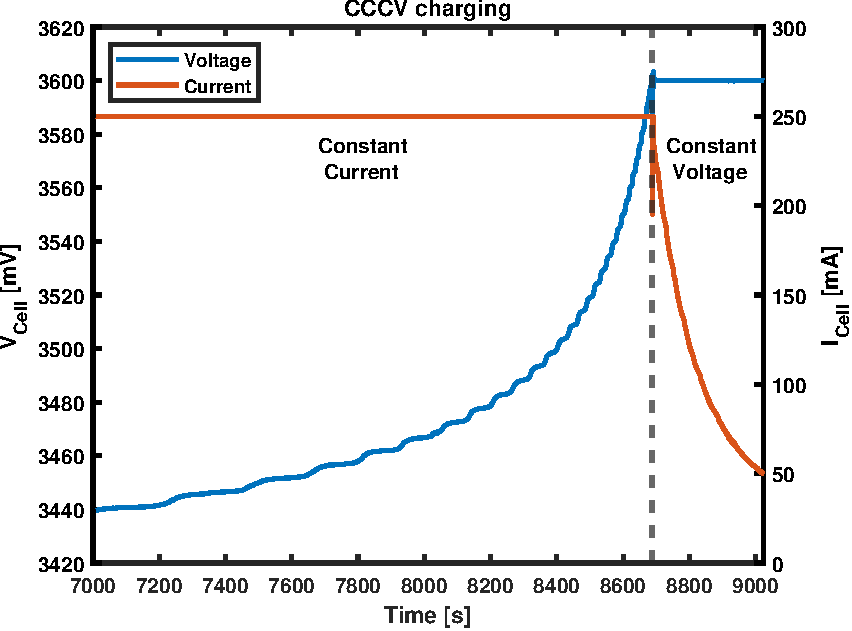
\includegraphics[width=\textwidth]{CCCV.pdf}
    \caption{Constant Current - Constant Voltage Charge}
    \label{fig:TestCCCV}
  \end{minipage}
  \hfill
  \begin{minipage}[b]{0.47\textwidth}
    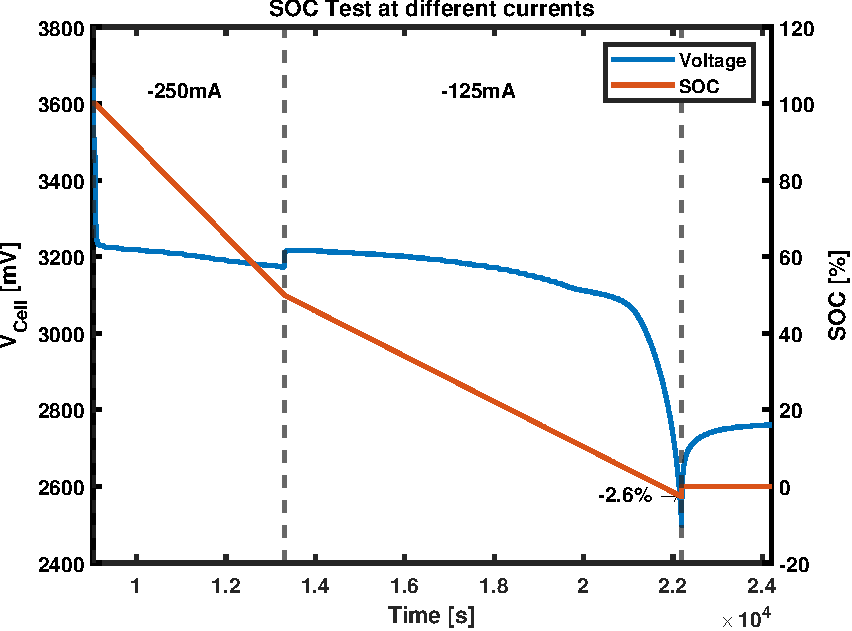
\includegraphics[width=\textwidth]{SOC.pdf}
    \caption{SOC discharge at different currents}
    \label{fig:TestSOC}
  \end{minipage}
\end{figure}

\begin{figure}[hbt!]
  \begin{minipage}[b]{0.44\textwidth}
    \centering
    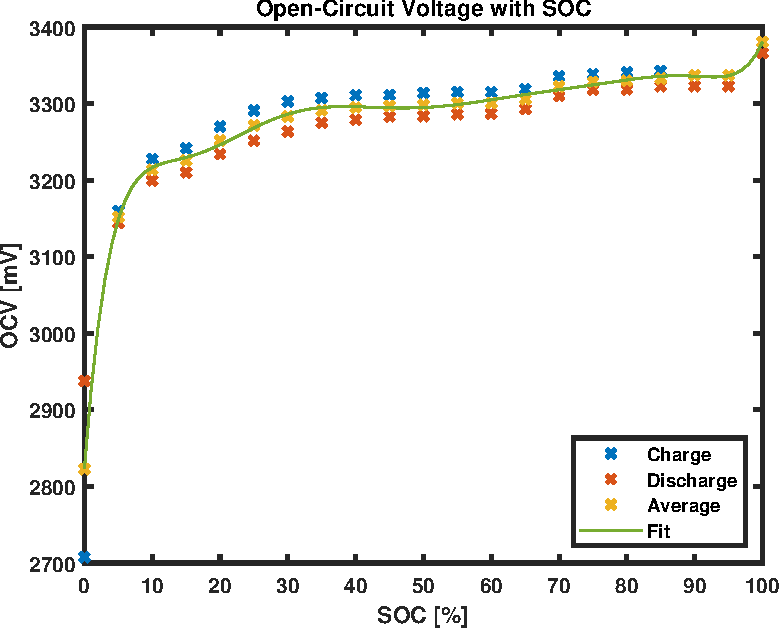
\includegraphics[width=\textwidth]{SOC_OVC.pdf}
    \caption{Relationship between SOC and OVC}
    \label{fig:SOC_OCV}
  \end{minipage}
  \hfill
  \begin{minipage}[b]{0.47\textwidth}
    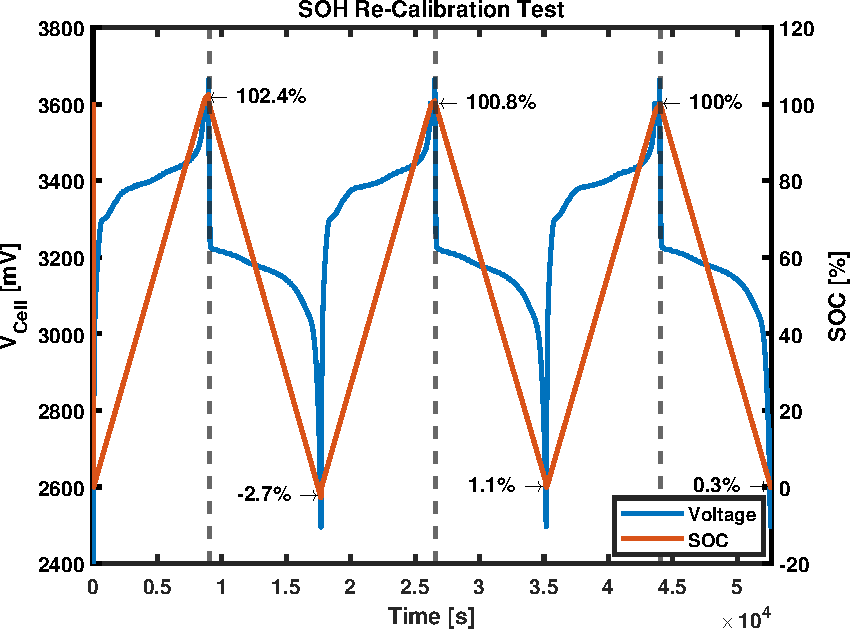
\includegraphics[width=\textwidth]{SOHTest.pdf}
    \caption{Testing SOH Re-calibration}
    \label{fig:SOHTest}
  \end{minipage}
\end{figure}

As stated during the Design Implementation, the initial value of the SOC is found using a lookup table of a pre-made SOC-OCV graph shown in figure \ref{fig:SOC_OCV} (There is a direct relationship between open-circuit voltage and state of charge). This was used in combination with linear interpolation within the Arduino to estimate the value of the starting SOC. Note however the uniform nature of the curve and the hysteresis caused by charging/discharging. This has created a significant amount of error due to an average having to be used. In addition to this, the quantization error of the Arduino is ($\sfrac{4}{2^{10}} = 3.9mV$), in some cases, larger than the difference in voltage between two 5\% intervals. This ultimately led to the decision to zero the Coulomb count the moment the cell is fully charged/ discharged. The Re-Calibration of the SOH is an integral part of the system in order to keep an accurate value of the SOC. This was tested by going through three charge-discharge cycles and allowing the Arduino to calibrate the SOH between each one. Figure \ref{fig:SOHTest} shows how well this worked with the error at each end decreasing to 0.03\% during charging and 0.3\% for the discharge. When testing the balancing, a simple discharge of two cells was implemented (Figure \ref{fig:TestDissipation}) with the gap between the SOCs correctly converging to 3\%. Having tested how the SOH re-calibration positively effects the coulomb count, it would make sense to decrease the balancing tolerance to a lower value like 0.3\% as the number of complete charge/discharge cycles increases.

\begin{figure}[hbt!]
  \begin{minipage}[b]{0.44\textwidth}
    \centering
    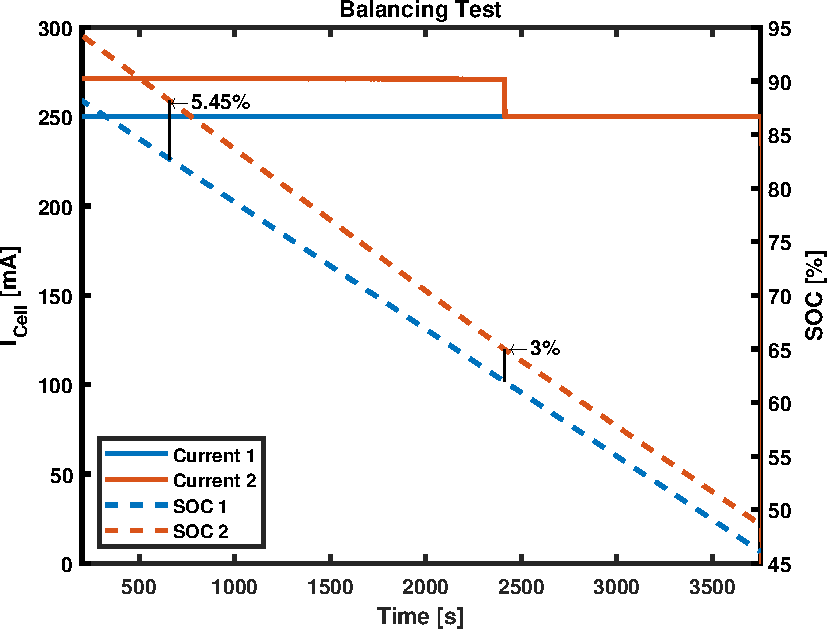
\includegraphics[width=\textwidth]{Dissipate.pdf}
    \caption{Relationship between SOC and OVC}
    \label{fig:TestDissipation}
  \end{minipage}
  \hfill
  \begin{minipage}[b]{0.47\textwidth}
    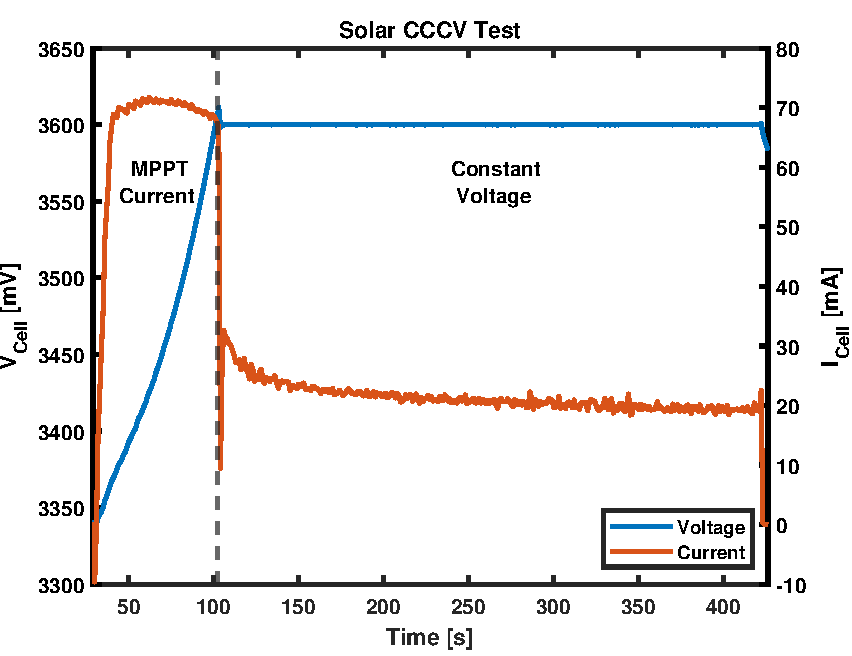
\includegraphics[width=\textwidth]{PVCCCV.pdf}
    \caption{Testing CCCV charging with PV}
    \label{fig:CCCVPV}
  \end{minipage}
\end{figure}

\subsubsection{PV Testing}

A single PV panel was first characterised to give a baseline for the MPPT program. In line with the theory, a single panel had a flat current-voltage curve until a breakdown voltage was reached (Figure \ref{fig:PVvoltage}). This breakdown voltage decreased as the PV cell was under the lamp for longer. Clearly, this is because temperature has increased and resulting in a lower peak for the power curve. The MPPT was then tested with a 2x2 panel arrangement in direct sunlight (Figure \ref{fig:TestMPPT}). In this case, the MPPT is looking at the voltages and currents at the output of the buck SMPS. This was done as the efficiency of the SMPS is likely to effect the shape of the power curve. Left-side tracking worked well with bigger intervals when the system was far away from the peak and smaller ones taken near it (Note the big clump of data points). This made sure that the fluctuations at the peak were minimal. Note that the right-sided tacking made it to the peak but took longer to do so. This seems like an extreme case where the gradient turns positive on the right-hand side; it is unlikely that it would ever get this bad but caution is advised. This may be an consequence of the $\sim 8V$ limitation of Port A on the SMPS causing shoot through between the PV Panel and the load. 

\begin{figure}[hbt!]
  \begin{minipage}[b]{0.47\textwidth}
    \centering
    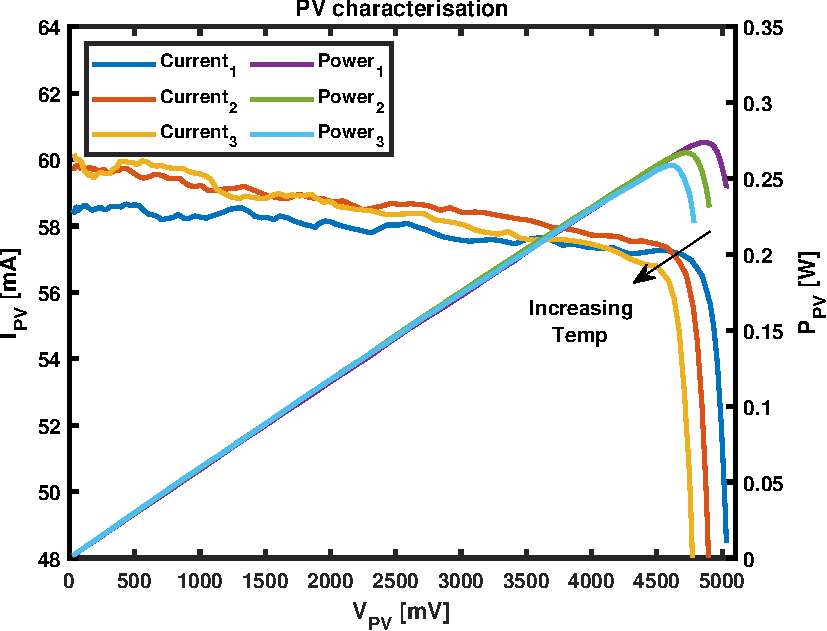
\includegraphics[width=\textwidth]{PVCombined.pdf}
    \caption{PV Current Characterisation}
    \label{fig:PVvoltage}
  \end{minipage}
  \hspace{0.8cm}
  \begin{minipage}[b]{0.44\textwidth}
    \includegraphics[width=\textwidth]{MPPT.pdf}
    \caption{2x2 PV MPPT Test under normal sunlight }
    \label{fig:TestMPPT}
  \end{minipage}
\end{figure}


\subsection{Vision}
I will be testing the subsystem according to the design criteria laid out in the problem definition and design criteria of vision section. Each criteria will be assessed and evaluated to determine whether it has been met and what could be done further to meet it. 

\textbf{Ball Detection Testing: }

To collect this I had to use a black background for the coloured balls and a white background for the black ball. I examined the output streams of each. I found that a camera gain of 0 was the preferable test setting also. 

\begin{figure}[hbt!]
    \centering
    \includegraphics[scale=0.6]{BallDetectNon.PNG}
    \captionsetup{justification=centering}
    \caption{Ball detection : Video Input , Green Detect , Pink Detect , Blue Detect , Orange Detect}
\end{figure}


\begin{figure}[hbt!]
    \centering
    \includegraphics[scale=0.4]{BlackBallDetect.PNG}
    \captionsetup{justification=centering}
    \caption{Black ball detection}
\end{figure}

\textit{Criteria one and Criteria two} are shown to be operational for all balls in stated conditions. The highlighting was unique to each ball, it was however susceptible to differing brightness conditions which meant the gain of the camera had to be adjusted to a low value. Further to this without a solid background the possibility for the incorrect highlighting of colour or unexpected brightness in the background was greater so often a solid background was required for testing. 
\textit{Criteria three} is Shown to work in the filter implementation which removed non constant white horizontals , I found that sometimes the image sometimes showed reduced noise occurring. This means I should increase the size of my noise filtering buffer to further increase the intensity of noise reduction. However it worked satisfactorily for non-reflective backgrounds. 
\textit{Criteria Four : } Can be seen from testing images ymin ymax and xmin xmax matching our ball highlighted pixels. Further testing of the distance calculated was done in command testing.


\textbf{Edge Detection Testing: }

The aim of this section was to detect obstructions from unknown visual data . I tested this section by observing a range of objects in front of the and moving them backwards and forwards in front of the camera. In both the sideways and upright camera mode.

\begin{figure}[hbt!]
    \centering
    \includegraphics[scale=0.3]{VerticalOrientEdge.PNG}
    \captionsetup{justification=centering}
    \caption{Vertical Camera position analysis}
\end{figure}

\begin{figure}[hbt!]
    \centering
    \includegraphics[scale=0.295]{HorizontalOrientEdge.PNG}
    \captionsetup{justification=centering}
    \caption{Horizontal oriented camera analysis}
\end{figure}

\textit{Criteria One : } We can see that depending on the orientation of the camera either vertical or horizontal edges are highlighted the Horizontally oriented camera analysis figure reveals the horizontal edges and was the orientation used in our final design. \textit{Criteria Two : } was successfully accomplished the the sectioning and average white pixel  position calculation in that section to give can be seen further in command implementations algorithms to find depth. 

\textbf{Communication Testing: }

This sections aim was to Relay information on detected objects to Control subsystem for further processing . To test its function I printed the received byte values on the serial monitor of the Arduino ESP it was connected to. I measured their accuracy and consistency by comparing the expected value to the received across multiple messages. 

\textit{Criteria One : } Shown to  be met by the inclusion of our array of registers :  \mintinline{verilog}{reg [7:0]mem[96:0];} , storing all data of from analysis of current frame. \textit{Criteria Two : } We can see the format in both the vision and control implementations but a summary can be seen below alongside an annotated serial monitor output of the Arduino : Thus we can see an see this criteria is satisfactorily met. \textit{Criteria Three : } The figure below reveals our data is received in the intended format with values associated to what we expect this consistently occurred across messages during testing. Further to this to ensure a robust design we implemented safeguards on the command subsystem which sanity check data before using it. Thus we can safely say the relayed data is accurate. 

\begin{figure}[hbt!]
  \begin{minipage}[b]{0.44\textwidth}
    \centering
    \includegraphics[scale = 0.5]{memoryMap.jpg}
    \caption{Memory map for communication to Control subsystem}
    \label{fig:mem_Map}
  \end{minipage}
  \hfill
  \begin{minipage}[b]{0.44\textwidth}
    \includegraphics[scale = 0.35]{Serial.jpg}
    \caption{Annotated Serial output of Arduino}
    \label{fig:SerialOut}
  \end{minipage}
\end{figure}

\subsection{Command}
\subsubsection{Testing Communication}
The communication through the API was tested using the "postman" app for HTTP requests. This application makes it easy to send POST and GET requests. The results of sending different fake rover movements and the resulting move commands from the server could easily be tested to ensure that the data was as expected. This also made it easier to work on the command system independently from the control system. Each of the three command modes was tested this way to ensure they gave the expected behaviour. The data sent to the interface could also be check for validity in different situations. The actual movement testing is discussed in the drive section.

\subsubsection{Testing Ball Positions}
As previously discussed the "matplotlib" python library was used for testing the map to ensure that the data looked roughly as expected, however it was also necessary to check the data numerically. The position of the balls on the server was checked to be as expected numerically after several movements and rotations were sent to the command system. The balls were also checked to be tracked as expected in all of the four quadrants of the map to ensure that the conversion between Cartesian and polar coordinates was correct. When first testing considerable errors were found when the ball was near the edge of the screen or too close to the rover. The was caused by the ball being only half on the screen and so the ball data was checked against certain conditions to ensure both edges were far enough within the field of view before using the data. We then tested the accuracy of the distance measurements, to test this balls were placed on marked positions in front of a solid background and the depth calculation result was read from the interface. We found that the when the ball was closer than 12cm to the camera the ball went over the edges of the camera view resulting in a distorted distance calculation. Due to this balls that were calculated to be within this margin are rejected by the server. It was also found that balls less well defined by the hue space had greater errors, this matched the results in vision testing where we can see the highlighting for blue and pink is less effective. The results of this testing can be seen in table \ref{tab:BallDistanceTest}.

\begin{table}[hbt]
\centering
\begin{tabular}{ |c||p{1cm}|p{1cm}|p{1cm}||p{1cm}|p{1cm}|p{1cm}||c|  }
 \hline
 Ball Colour & \multicolumn{3}{|c||}{Actual Distance (cm)} &  \multicolumn{3}{|c||}{Calculated Distance (cm)} & Error\\
 \hline
 Blue & 15 &30 &50 & 19 & 36 & 60 & 21\% \\
 Green & 15 & 30 & 50 & 16 & 32 & 56 & 9\% \\
 Black & 15 & 30 & 50 & 14 & 33 & 59 & 11\% \\
 Orange & 15 & 30 & 50 & 17 & 35 & 55 & 12\% \\
 Pink & 15 & 30 & 50 & 20 & 39 & 62 & 27\% \\
 \hline
\end{tabular}
\caption{\label{tab:BallDistanceTest} Average Error of Ball Position at Different Distances}
\end{table}
\subsubsection{Testing Depth Detection}
In testing the depth detection algorithm we were unable to get a smooth estimator of depth in many directions. We were able to detect if an object was moving directly towards the rover, which is still useful in notifying the user of a potential collision. An example of this working can be seen in the video at time 1:18. 

\subsubsection{Testing Speed of Move Generation}
The speed of the server to make a movement decision in each of the three modes, not including the time taken to reach control was tested to ensure that the delay was acceptable. The tests were taken as an average of running the move creation 10000 times with random inputs to the system. The results from the testing are in table \ref{tab:MoveGeneration}. As can be seen the creation of one movement took in the order of 100th of a millisecond which is a negligible amount of time next to the delay in the transfer of information over the internet
\begin{table}[hbt]
\centering
\begin{tabular}{ |p{3cm}||p{3cm}|p{3cm}|p{3cm}|  }
\hline
 Mode & Command & Map & Search\\
 \hline
 Time (s)  & 0.06    &A 0.24 &   0.31\\
 \hline
\end{tabular}
\caption{\label{tab:MoveGeneration} Total Time to Generate 10000 Moves}
\end{table}

\subsubsection{Testing Obstacle Avoidance}
The obstacle avoidance system was tested with multiple balls and routes to ensure that the main functionality was working correctly, which it was found to be. The obstacle avoidance was also tested separately from the actual rover using a function for printing the map and the route adapted from the sources used \cite{AAB}\cite{ImplementationA}. We then decided to test the speed of the two different algorithms for finding the optimal route, Dijkstra and A-Star. Table \ref{tab:MoveGeneration} shows the results from testing the two modes with varying number of balls. As can be seen there is no real time difference between the two options within this ball range. As the maximum number of balls we have is 5 either option is clearly fine.
\begin{table}[hbt]
\centering 
\begin{tabular}{ |p{3cm}||p{3cm}|p{3cm}|  }
 \hline
 Mode & Number of Balls & Time (ms) \\
 \hline
 Dijkstra & 50   & 0.018\\
 A-Star & 50   & 0.016\\
 Dijkstra & 70   &0.043\\
 A-Star & 70   &0.046\\
 Dijkstra & 100 &0.062\\
 A-Star & 100   &0.078\\
 Dijkstra & 150   &0.080\\
 A-Star & 150   &0.091\\
 \hline
\end{tabular}
\caption{\label{tab:Optimal Route} Time Taken To Find Optimal Route}
\end{table}


\subsection{Control}
Two different testing strategies have been adopted to ensure proper functioning of the Control subsystem
\paragraph{Qualitative testing} Communication between Control and any other subsystem has been tested in the following way:
\begin{itemize}[nolistsep]
    \item The receiver subsystem and the transmitter subsystem were connected by the chosen communication protocol. (In the case of bidirectional communication their role would be interchanged in order to test the communication in the opposite direction)
    \item The transmitter would send mock data over the communication protocol
    \item It was checked that the data received by the receiver matched with the mock data sent by the transmitter. Adjustments were made if this was not the case.
\end{itemize}

The full communication flow was tested by giving instruction to the Rover using the remote UI and checking that it would behave as expected.

\paragraph{Quantitative testing}
Each communication protocol (UART, SPI, HTTP) has been tested and evaluated according to two parameters
\begin{itemize}
    \item error rate, in order to asses the \emph{reliability} of the communication
    \item speed of data transmission, in order to asses whether the communication is \emph{fast} enough
\end{itemize}

The error rate has been measured in the following way:
\begin{itemize}[noitemsep]
    \item a receiver and a transmitter have been connected using UART, SPI and HTTP GET and POST
    \item the transmitter sends an array of known data
    \item the receiver collects the data and counts the number of times the wrong number has been received
\end{itemize}

No error was detected in any of the tests run, which brought us to the conclusion that the communication protocols were reliable enough for the given application.
\smallskip
The speed of data transmission for UART and SPI can be adjusted to meet the design criteria by picking an appropriate baud-rate and selecting a clock divider for UART and SPI communication respectively.
The speed of data transmission for HTTP over WiFi has been measured by sending messages with a fixed payload and measuring the average delay for the full data transmission.

\begin{table}[hbt]
\centering
\renewcommand{\arraystretch}{1.3}
\begin{tabular}{@{}ll@{}}
\toprule
Communication   Protocol & Speed of data   transmission \\ \midrule
UART                     & 115200 bits/s                \\
SPI                      & 2000000   bits/s             \\
HTTP                     & 70 ms latency                  \\ \bottomrule
\end{tabular}
\caption{Speed of Transmission}
\end{table}

\subsection{Integration}
Throughout the development and implementation processes of the modules, 





\newpage
\section{Evaluation and Critical analysis}
\textbf{Drive Final evaluation:} The drive unit implementation was satisfactory both in terms of functionality and performance: additional features were successfully implemented such as the option to tune the speed and the alternative back-up algorithm for when the optical sensor is unreliable. However, the decision of sending the location information very frequently caused small delays throughout the movements. This could have been improved by speeding up the communication or continuing with the execution of the instruction while communication with the server, although this would have made the location data less accurate. Another feature that could have improved the quality of the movements would have been to implement a mathematical model to compute the optimal trajectory following an arch, in order to make the movements look smoother (e.g. doing the spiral to search for balls). This have been discarded for the huge complexity that would have involved, given that the precision and speed were our priorities. Overall, the performance was within the 10\% error required and in the end the only relevant limitations were caused by the hardware components we could not substitute (e.g. optical sensor).

\textbf{Energy Final evaluation:} Though the criteria for the Energy subsystem is clearly defined, there are multiple ways the specification could have been satisfied with varying degrees of success. A main challenge in getting an accurate SOC and SOH estimation has been dealing with the quantization error of the analogue ports. The moving average filter has worked well in mitigating this but a highly accurate system would require a Kalman filter. This was not used as it is computationally extensive, though it could have been offloaded to Control. Having an estimate of the current on the other side of the SMPS is also not ideal and in the future this should be accounted for. An MPPT algorithm based upon Incremental Conductance worked well in most conditions but, as seen during testing, it struggled if the slope was near vertical. A perturb and observe method may have worked better with this extreme case. Overall, the system met the specification set but a main problem would be the capacity as only 2 cells are in use. This unfortunately is a limitation of the SMPS and a possible solution would be to have the cells in a 2x2 configuration. This would however compromise on safety due to unwanted auto balancing between the cells. 

\textbf{Vision Final evaluation:} I was happy the design criteria of my subsystem were mostly met by the final implementation. The edge detection process successfully allowed for unidentified (Non ball) objects to be detected and displayed which was a great success. However I would aim for further noise elimination or a higher tolerance for edge high-lighting as it was very susceptible to differing brightness and shadowing on flat surfaces.  Ball detection was again a robust process for colours such as green ,orange, blue, red (All well-defined hue spaces) but adjusting of the camera gain and environment was required to isolate the black ball. Further to this, if a significant amount of constant colour existed, it could affect the detection to tackle this. I would develop a more advanced elimination of non-ball highlighting. Overall the vision system achieved its high-level objectives for obstacle avoidance and target identification. 

\textbf{Control Final evaluation:} Although the design criteria for the Control subsystem were met, a few improvements could be made to improve the communication design. The obstacle avoidance algorithm could have been implemented locally on the ESP32. In this way the delay introduced by continuously exchanging data with the Server to receive the next move could have been removed. Furthermore, WebSockets could have been used instead of HTTPS to reduce the latency for wireless communication with the Server.

\textbf{Command Final evaluation:} The command subsystem met the desired requirements in terms of providing all the information necessary to the user and creating commands to send to the rover. Several features were successfully implemented as well as possible with the data available, such as terrain mapping, depth estimation and the ability to search for balls. The obstacle avoidance system, whilst functioning as expected could have been improved by adding an estimation of terrain suitability to find a better path. It could also have been improved by changing the way the graph is constructed to only contain nodes next to obstacles to increase speed of computation and find a more optimal route. 

\textbf{Rover Final evaluation:} The final version of the rover system achieved all requirements outlined in the project brief - the rover successfully achieved communication with the server, detected the coloured balls and avoided them. On top of the basic criteria, several additional functions and more sophisticated implementations were developed and implemented in the final rover. This includes the use of edge detection in the Vision module to detect non-ball objects; the spiral motion used to search for the balls in the autonomous mode implemented by Command; the bi-directional communication between the Control and Energy modules.


\newpage
\section{Essay 'Intellectual Property'}

Intellectual property (or IP) refers to the ownership of a creation by the person who created it. \cite{WhatProperty} It is an intangible asset that can be bought or sold. Various types of intellectual property rights exist that allow the owner to stop others from using or copying their work. In the development of a new product, it is extremely important to understand the laws on IP in the countries you plan to publish your creation and to consider applying for IP rights as early on as possible. It is also important to carry out research on the intellectual property held by others in the same sector to avoid  IP infringement.

The main types of IP rights are copyright, design rights, trademarks and patents. \cite{IntellectualGOV.UK} For copyright, unregistered design rights and unregistered trademarks, no application has to be made as these rights apply automatically. However, in order to report infringement for these rights, proof must be provided of the product, work or branding being used or copied. For registered design rights, registered trademarks and patents, applications must be made in order to obtain the rights. In these cases, proof is not required to report infringements. However, registered rights need capital and time – in particular, obtaining patents can cost thousands of pounds and the application can take several years to obtain.  

Copyright protects creative expression and in the context of the Mars Rover, would automatically apply to all original software developed for the project. For code that has been used or adapted from others, we would need to reach out to and come to an agreement with the authors of that code before publishing or using commercially. Design rights protect the appearance of the product and for the Mars Rover, it would refer to the specific arrangement of the rover modules. In this case, the design rights would belong to the department who came up with the original design for the rover. Trademarks protect branding, and would be important if we decided to start a business to commercialise the rover. Patents protect inventions and products and in the case of the rover, could be applied to things such as, if the energy module discovered a method that draws power more efficiently from the solar panels. Patents must be applied for before the invention is published and so it is imperative that an IP attorney are considered at an early stage of the invention. 




\newpage
\begin{appendices}

\section{Energy}

\setcounter{figure}{0}  %Resets the figure count
\setcounter{table}{0}   %Resets the table count

\begin{figure}[htb]
    \centering
    \includegraphics[width = \textwidth]{FinalCircuit.pdf}
    \caption{Complete Circuit}
    \label{fig:FinalCircuit}
\end{figure}

\begin{table}[htb]
    \centering
    \renewcommand{\arraystretch}{1.3}
    \begin{tabular}{||c|c|c||}
    \hline
    Specification & Value & Unit \\ [0.5ex]
    \hline \hline
    Nominal Voltage    & 3.2 & V\\
    Nominal Capacity     & 500 & mAh\\
    Minimum Voltage         & 2  & V\\
    Charging Method     & CC/CV 3.6  & V\\
    Standard Charging Current CC    & 250  & mA\\
    Continuous Discharge Current   & 500  &   mA\\
    \hline
    \end{tabular}
    \caption{Cell Specification \quad Source: Adapted from \cite{AmpsplusBattery}}
    \label{fig:CellSpecification}
\end{table}
\label{appendix:Energy}

\begin{table}[htb]
    \centering
    \renewcommand{\arraystretch}{1.3}
    \begin{tabular}{||c|c|c||}
    \hline
    Specification & Value & Unit \\ [0.5ex]
    \hline \hline
        Voltage  & 5 & V\\
        Current & 230 & mA\\
        Power & 1.15 & W \\
        Power Tolerance & +/-3 & \% \\
        Temperature Coefficient & -0.45 & $^{\circ} C$ \\
        \hline
    \end{tabular}
    \caption{PV Specifiation \quad Source: Adapted from \cite{NoTitle}}
    \label{tab:PVSpecification}
\end{table}



\newpage
\section{Command}

\setcounter{figure}{0}  %Resets the figure count
\setcounter{table}{0}   %Resets the table count

\end{appendices}

\bibliographystyle{IEEEtranN}
\bibliography{references.bib, referencesams.bib}












\end{document}
